\documentclass[9pt,preprint]{sigplanconf}
\usepackage{amsmath}
\usepackage{amssymb} 
\usepackage{amsthm}
\usepackage{ stmaryrd }
\usepackage{mathpartir}
%\usepackage{cite}
%\renewcommand{\citepunct}{,\,} % IEEEtran wants to use ],\,[ for this but that looks dumb...

\newcommand{\atlam}{@$\lambda$}

% Generic
\newcommand{\bindin}[2]{#1;~#2}
\newcommand{\pipe}{~\text{\large $\vert$}~}
\newcommand{\splat}[3]{#1_{#2};\ldots;#1_{#3}}
\newcommand{\splatC}[3]{#1_{#2}~~~~\cdots~~~~#1_{#3}}
\newcommand{\splatTwo}[4]{#1_{#3}#2_{#3},~\ldots~, #1_{#4}#2_{#4}}
\newcommand{\substn}[2]{[#1]#2}
\newcommand{\subst}[3]{\substn{#1/#2}{#3}}
\newcommand{\entails}[2]{#1 \vdash #2}

% Programs
\newcommand{\progsort}{\rho}
\newcommand{\pfam}[2]{\bindin{#1}{#2}}
\newcommand{\pdef}[4]{\bindin{{\sf def}~\tvar{#1}:#2=#3}{#4}}

% Families
\newcommand{\fvar}[1]{\textsc{#1}}

\newcommand{\family}[6]{{\sf family}~\fvar{#1}[#2]\sim \tvar{#5}.#6~\{#3\}}
\newcommand{\familyDf}{\family{Fam}{\kappaidx}{\opsort}{\opsigsort}{i}{\taurep}}

% Operators
\newcommand{\opsort}{\theta}
\newcommand{\opsigsort}{\Theta}
\newcommand{\opvar}[1]{\textbf{\textit{#1}}}

% Expressions
\newcommand{\evar}[1]{#1}
\newcommand{\elam}[3]{\lambda #1{:}#2.#3}
\newcommand{\eapp}[2]{{#1~#2}}
\newcommand{\eopapp}[2]{\eop{Arrow}{ap}{\tunit}{#1; #2}}
\newcommand{\eop}[4]{{\fvar{#1}.\opvar{#2}\langle#3\rangle(#4)}}
\newcommand{\elet}[4]{{\sf let}~#1 : #2 = #3~{\sf in}~#4}

% Type-Level Terms
\newcommand{\tvar}[1]{{\textbf{#1}}}

\newcommand{\tlam}[3]{\lambda \tvar{#1}{:}{#2}.#3}
\newcommand{\tapp}[2]{#1~#2}
\newcommand{\tifeq}[5]{{\sf if}~#1\equiv_{#3}#2{\sf ~then~}#4~{\sf else}~#5}
\newcommand{\tstr}[1]{\textit{``#1''}}
\newcommand{\tunit}{()}
\newcommand{\tpair}[2]{(#1, #2)}
\newcommand{\tfst}[1]{{\sf fst}(#1)}
\newcommand{\tsnd}[1]{{\sf snd}(#1)}
\newcommand{\tnil}[1]{[]_#1}
\newcommand{\tcons}[2]{#1 :: #2}
\newcommand{\tfold}[6]{{\sf fold}(#1; #2; \tvar{#3},\tvar{#4},\tvar{#5}.#6)}

\newcommand{\tfamSpec}[5]{{\sf family}~[#2]~::~#3~\{#4 : #5\}}
\newcommand{\tfamSpecStd}{\tfamSpec{fam}{\kappaidx}{\taurep}{\theta}{\Theta}}

\newcommand{\ttype}[2]{\fvar{#1}\langle#2\rangle}
\newcommand{\ttypestd}{\ttype{Fam}{\tau}}
\newcommand{\tfamcase}[5]{{\sf case}~#1~{\sf of}~\fvar{#2}\langle\tvar{#3}\rangle\Rightarrow#4~{\sf ow}~#5}
\newcommand{\trepof}[1]{{\sf rep}(#1)}

\newcommand{\tden}[2]{\llbracket #1~{\sf as}~#2 \rrbracket}
\newcommand{\ttypeof}[1]{{\sf typeof}~#1}
\newcommand{\tvalof}[2]{{\sf trans}(\tden{#1}{#2})}
\newcommand{\terr}{{\sf err}}
\newcommand{\tdencase}[5]{{\sf case}~#1~{\sf of}~\tden{\tvar{#2}}{\tvar{#3}}\Rightarrow#4~{\sf ow}~#5}

\newcommand{\titerm}[1]{\triangledown(#1)}
\newcommand{\titype}[1]{\blacktriangledown(#1)}

\newcommand{\tconst}[1]{{\sf const}(#1)}
\newcommand{\tOp}[1]{{\sf op}(#1)}

\newcommand{\tprog}[1]{{\sf program}(#1)}

\newcommand{\topsempty}{\cdot}
\newcommand{\tops}[5]{\opvar{#1}[#2](\tvar{#3},\tvar{#4}.#5)}
\newcommand{\topp}[2]{#1; #2}
\newcommand{\Tops}[2]{\tvar{#1} : #2}
\newcommand{\Topp}[2]{#1; #2}
\newcommand{\kOpEmpty}{\cdot}
\newcommand{\kOpS}[2]{\opvar{#1}[#2]}
\newcommand{\kOp}[3]{#1; \kOpS{#2}{#3}}

% Contexts
\newcommand{\fCtx}{\Sigma}
\newcommand{\itvarCtx}{\Omega}
\newcommand{\iCtx}{\Theta}
\newcommand{\eCtx}{\Gamma}
\newcommand{\etvarCtx}{\Omega}
\newcommand{\errCtx}{\mathcal{E}}
\newcommand{\famEvalCtx}{\Xi}

% Judgments
\newcommand{\emptyctx}{\emptyset}
\newcommand{\tvarCtx}{\Delta}
\newcommand{\tvarCtxX}[2]{\Delta, {\tvar{#1}} : {#2}}
\newcommand{\fvarCtx}{\Sigma}
\newcommand{\fvarCtxX}{\Sigma, \fvarOfType{Fam}{\kappaidx}{\Theta}}
\newcommand{\eivarCtx}{\Omega}
\newcommand{\eivarCtxX}[1]{\Omega, \evar{#1}}

\newcommand{\kEntails}[3]{#1 \vdash_{#2} #3}

\newcommand{\progProg}[1]{#1~{\tt prog}}
\newcommand{\progOK}[3]{\kEntails{#1}{#2}{\progProg{#3}}}
\newcommand{\progOKX}[1]{\progOK{\tvarCtx}{\fvarCtx}{#1}}

\newcommand{\fvarOfType}[3]{\fvar{#1}[#2,#3]}
\newcommand{\fvarOfTypeDf}{\fvarOfType{Fam}{\kappaidx}{\Theta}}

\newcommand{\opOfType}[2]{#1 : #2}
\newcommand{\opType}[4]{\kEntails{#1}{#2}{\opOfType{#3}{#4}}}

\newcommand{\tOfKind}[2]{#1 : #2}
\newcommand{\tKind}[4]{\kEntails{#1}{#2}{\tOfKind{#3}{#4}}}
\newcommand{\tKindX}[2]{\tKind{\tvarCtx}{\fvarCtx}{#1}{#2}}

\newcommand{\isExpr}[1]{#1~\texttt{expr}}
\newcommand{\exprOK}[4]{#1~#2 \vdash_{#3} \isExpr{#4}}
\newcommand{\exprOKX}[1]{\exprOK{\tvarCtx}{\eivarCtx}{\fvarCtx}{#1}}

\newcommand{\isIterm}[4]{#1~#2 \vdash_{#3} #4~\texttt{iterm}}
\newcommand{\isItermX}[1]{\isIterm{\tvarCtx}{\eivarCtx}{\fvarCtx}{#1}}

\newcommand{\isItype}[3]{#1 \vdash_{#2} #3~\texttt{itype}}
\newcommand{\isItypeX}[1]{\isItype{\tvarCtx}{\fvarCtx}{#1}}

\newcommand{\tEvalX}[2]{#1 \Downarrow #2}
\newcommand{\tiEvalX}[2]{#1 \curlyveedownarrow #2}

\newcommand{\fvalCtx}{\Phi}
\newcommand{\fvalCtxX}[1]{\Phi, #1}
\newcommand{\fval}[4]{\fvar{#1}[#2, \tvar{#3}.#4]}
\newcommand{\fvalDf}{\fval{Fam}{\theta}{i}{\tau}}

\newcommand{\pcompiles}[3]{\vdash_{#1} #2 \Longrightarrow #3}
\newcommand{\pcompilesX}[1]{\pcompiles{\fvalCtx}{#1}{\gamma}}

\newcommand{\ptcc}[2]{#1 \longrightarrow #2}

\newcommand{\etCtx}{\Gamma}
\newcommand{\etCtxX}[2]{\etCtx, \evar{#1} : #2}

\newcommand{\gtCtx}{\Psi}
\newcommand{\gtCtxX}[2]{\gtCtx, \evar{#1} : #2}

\newcommand{\ecompiles}[5]{#1 \vdash_{#2} #3 : #4 \Longrightarrow #5}
\newcommand{\ecompilesX}[3]{\ecompiles{\etCtx}{\fvalCtx}{#1}{#2}{#3}}

\newcommand{\delfromtau}[4]{\vdash^{\fvar{#1}}_{#2} #3 \sim #4}
\newcommand{\tauisdel}[5]{\vdash^{\fvar{#1}}_{#2} \ttype{#3}{#4} \sim #5}

\newcommand{\checkRC}[5]{#1 \vdash^{\fvar{#2}}_{#3} #4 \sim #5}
\newcommand{\checkRCX}[2]{\checkRC{\gtCtx}{Fam}{\fvalCtx}{#1}{#2}}

\newcommand{\erase}[3]{\vdash_{#1} #2 \leadsto #3}
\newcommand{\eraseX}[2]{\erase{\fvalCtx}{#1}{#2}}

\newcommand{\eCtxTogCtx}[4]{\vdash^{\fvar{#1}}_{#2} #3 \sim #4}
\newcommand{\eCtxTogCtxX}[2]{\eCtxTogCtx{Fam}{\fvalCtx}{#1}{#2}}

\newcommand{\ddbar}[4]{\vdash^{\fvar{#1}}_{#2} #3 \sim #4}
\newcommand{\ddbarX}[2]{\ddbar{Fam}{\fvalCtx}{#1}{#2}}

\newcommand{\iType}[3]{#1 \vdash #2 : #3}

\newcommand{\gtCtxH}{\hat{\gtCtx}}
\newcommand{\gtCtxHX}[2]{\gtCtxH, \evar{#1} : #2}

%
\newcommand{\fSpec}[3]{\tof{\fvar{#1}}{\kFam{#2}{#3}}}
\newcommand{\fSpecStd}{\fSpec{fam}{\kappaidx}{\Theta}}

% \tau
\newcommand{\taut}[1]{{\tau_{\text{#1}}}}
\newcommand{\tautype}{\taut{type}}
\newcommand{\tautrans}{\taut{trans}}
\newcommand{\tauproof}{\taut{proof}}
\newcommand{\tauidx}{\taut{idx}}
\newcommand{\taui}{\taut{i}}
\newcommand{\tauidxn}[1]{\taut{idx,#1}}
\newcommand{\taurep}{\taut{rep}}
\newcommand{\taurepn}[1]{\taut{rep,#1}}
\newcommand{\tauden}{\taut{den}}
\newcommand{\tauIT}{\taut{IT}}
\newcommand{\tauarrow}{\taut{arrow}}
\newcommand{\tauprod}{\taut{prod}}
\newcommand{\tauint}{\taut{int}}
\newcommand{\taubool}{\taut{bool}}
\newcommand{\tauprog}{\taut{prog}}
\newcommand{\tauiterm}{\taut{iterm}}
\newcommand{\tauval}{\taut{val}}
\newcommand{\tauop}{\taut{op}}

% \gamma
\newcommand{\ghat}{\hat{\gamma}}

% \sigma
\newcommand{\delt}[1]{\sigma_{\text{#1}}}
\newcommand{\delrep}{\delt{rep}}
\newcommand{\dhat}{\hat{\sigma}}
\newcommand{\dbar}{\bar{\sigma}}

% \kappa
\newcommand{\kappat}[1]{\kappa_{\text{#1}}}
\newcommand{\kappaidx}{\kappat{idx}}
\newcommand{\kappai}{\kappat{i}}

% Types

% IL terms
\newcommand{\ivar}[1]{\textrm{#1}}
\newcommand{\ilam}[3]{\lambda #1{:}#2.#3}
\newcommand{\ifix}[3]{{\sf fix~}#1{:}#2~{\sf is}~#3}
\newcommand{\iapp}[2]{#1~#2}
\newcommand{\ipair}[2]{(#1, #2)}
\newcommand{\ifst}[1]{{\sf fst}(#1)}
\newcommand{\isnd}[1]{{\sf snd}(#1)}
\newcommand{\iintlit}{\bar{
\textrm{z}}}
\newcommand{\iop}[2]{#1 \oplus #2}
\newcommand{\iIfEq}[5]{{\sf if}~#1\equiv_{#3}#2{\sf ~then~}#4~{\sf else}~#5}
\newcommand{\mvalof}[1]{{\sf valof}(#1)}
\newcommand{\iup}[1]{\vartriangle\hspace{-2.5pt}(#1)}

% Internal Types
\newcommand{\darrow}[2]{#1\rightarrow#2}
\newcommand{\dint}{\mathbb{Z}}
\newcommand{\dpair}[2]{#1\times#2}
\newcommand{\dup}[1]{\blacktriangle(#1)}
\newcommand{\drepof}[1]{{\sf repof}(#1)}

% Kinds
\newcommand{\kvar}[1]{\textrm{#1}}
\newcommand{\karrow}[2]{#1\rightarrow{#2}}
\newcommand{\kforall}[2]{\forall \kvar{#1}.#2}
\newcommand{\kstr}{\textsf{Str}}
\newcommand{\kunit}{\textsf{1}}
\newcommand{\kpair}[2]{#1 \times #2}
\newcommand{\klist}[1]{\textsf{list}[#1]}
\newcommand{\kTypeBlur}{\star}
\newcommand{\kDen}{\textsf{Den}}
\newcommand{\kIType}{\textsf{ITy}}
\newcommand{\kITerm}{\textsf{ITm}}

% Judgements
\newcommand{\tof}[2]{#1 : #2}
\newcommand{\mtof}[2]{#1 :: #2}
\newcommand{\tentails}[2]{#1 \vdash #2}
\newcommand{\tentailst}[3]{\tentails{#1}{\tof{#2}{#3}}}
\newcommand{\tStdCtx}{\fCtx~\tvarCtx}
\newcommand{\tCtxXF}[1]{\fCtx, #1~\tvarCtx}
\newcommand{\tCtxXT}[1]{\fCtx~\tvarCtx, #1}
%\newcommand{\tCtxXL}[1]{\fCtx~\tvarCtx~\lvarCtx, #1}
\newcommand{\tentailsX}[1]{\tentails{\tStdCtx}{#1}}
\newcommand{\tentailsXt}[2]{\tentailsX{\tof{#1}{#2}}}
\newcommand{\kentails}[2]{#1 \vdash #2}
\newcommand{\kentailsX}[1]{\kentails{\fCtx}{#1}}
\newcommand{\iMkCtx}[3]{#1~#2~#3}
\newcommand{\iStdCtx}{\iMkCtx{\fCtx}{\tvarCtx}{\itvarCtx}}
\newcommand{\ientails}[2]{#1 \vdash #2}
\newcommand{\ientailsX}[1]{\entails{\iStdCtx}{#1}}
\newcommand{\casemap}[2]{#1 : #2}
\newcommand{\mentails}[3]{#1, #2 \vdash #3}
\newcommand{\mentailsX}[1]{\mentails{\tvarCtx}{\itvarCtx}{#1}}
\newcommand{\eentails}[4]{#1~#2~#3 \vdash #4}
\newcommand{\eentailsX}[1]{\eentails{\fCtx}{\tvarCtx}{\etvarCtx}{#1}}
\newcommand{\mtentails}[2]{#1 \vdash #2}
\newcommand{\mtentailsX}[1]{\mtentails{\iCtx}{#1}}
\newcommand{\mtentailsXt}[2]{\mtentails{\iCtx}{\mtof{#1}{#2}}}
\newcommand{\kSimple}[1]{#1~{\sf simple}}
\newcommand{\Tentails}[3]{#1 \vdash_{#2} #3}
\newcommand{\TentailsX}[1]{\Tentails{\fCtx}{\fvar{fam}}{#1}}
\newcommand{\kEq}[1]{#1~\texttt{eq}}

% Verification and Translation
\newcommand{\translates}[4]{\entails{#1}{#2 \longrightarrow \tden{#3}{#4}}}

% Compilation Semantics
\newcommand{\compiless}[3]{#1 \Longrightarrow \tden{#2}{#3}}
\newcommand{\compiles}[3]{#1 \Longrightarrow \tden{#2}{#3}}
%\newcommand{\translates}[6]{\entails{#1}{\translatesTo{#2}{#3}{#4}{#5}{#6}}}
\newcommand{\translatesTo}[5]{#1 \longrightarrow \tden{#2}{\ttype{#3}{#4}{#5}{6}{7}}}
\newcommand{\translatesX}[5]{\translates{\eCtx}{#1}{#2}{#3}{#4}{#5}}


\renewcommand{\ttdefault}{txtt}
\usepackage{alltt}
\usepackage{listings}
\lstset{language=ML,
showstringspaces=false,
basicstyle=\ttfamily\footnotesize,
morekeywords={newcase,extends}}

\usepackage{float}
\floatstyle{ruled}
\newfloat{codelisting}{tp}{lop}
\floatname{codelisting}{Listing}

\newcommand{\compresslist}{
  \vspace{-1em}
  \setlength{\itemsep}{1pt}
  \setlength{\parskip}{0pt}
  \setlength{\parsep}{0pt}
}

\usepackage{url}
% url.sty was written by Donald Arseneau. It provides better support for
% handling and breaking URLs. url.sty is already installed on most LaTeX
% systems. The latest version can be obtained at:
% http://www.ctan.org/tex-archive/macros/latex/contrib/misc/
% Read the url.sty source comments for usage information. Basically,
% \url{my_url_here}.

\usepackage{placeins}

%\lefthyphenmin=4
\hyphenation{op-tical net-works semi-conduc-tor}

\usepackage{todonotes}

\lefthyphenmin=6

\begin{document}

\conferenceinfo{-}{-} 
\copyrightyear{-} 
\copyrightdata{[to be supplied]} 

%\titlebanner{{\tt \textcolor{Red}{{\small Under Review -- distribute within CMU only.}}}}        % These are ignored unless
%\preprintfooter{Distribute within CMU only.}   % 'preprint' option specified.

\title{Active Embeddings: Conservatively Extending a Type System From Within}

\authorinfo{Cyrus Omar\and Jonathan Aldrich}
           {Carnegie Mellon University}
            {\{comar, aldrich\}@cs.cmu.edu}   

\maketitle
\begin{abstract}
Researchers often need to extend an existing language with new type and operator constructors to realize a new abstraction in its strongest form. 
But this is not generally possible from within, so it is common to develop dialects and ``toy'' languages.
Unfortunately, taking this approach limits the utility of these abstractions: they cannot be imported by clients of other dialects and languages, and building applications where different components rely on different type systems is both unsafe and unnatural. 
%An {internally} {extensible} type system could help address these issues, but designing an extension mechanism that is both expressive and safe is non-trivial: extensions must not be permitted to compromise key metatheoretic properties of the language, nor should they be allowed to weaken one another, in any combination.

We introduce @$\lambda$, a simply-typed lambda calculus with simply-kinded type-level computation where new indexed type and operator constructors can be declared  from within. %It is structured in four layers: at the top-level, extension providers declare new indexed type constructors and term-level operator constructors. 
Type-level functions associated with operator constructors define their static and dynamic semantics, the latter by translation to a fixed typed internal language. By lifting compiler correctness techniques into the language, the ``actively typed semantics'' guarantees type safety. Going further, the semantics enforce an abstraction barrier at extension boundaries that ensures that extensions are mutually conservative (i.e. they do not weaken or interfere with one another, so that they can  be used together in any combination). 
%Totality of the type-level language guarantees decidability of type checking and equality constraints on type indices makes type equivalence decidable. 
We intend @$\lambda$ as a minimal foundation for future work on safe language-integrated extension mechanisms for typed programming languages, but it is already quite expressive. We demonstrate by showing how a conventional concrete syntax can be introduced by type-directed dispatch to Core @$\lambda$, then discuss a number of typed language fragments that can be \emph{actively embedded} by this mechanism as orthogonal ``libraries''. %(and discuss the sorts of fragments that, as yet, cannot).
\end{abstract}

%\category{D.3.2}{Programming Languages}{Language Classifications}[Extensible Languages]
%\category{D.3.4}{Programming Languages}{Processors}[Compilers]
%\category{F.3.1}{Logics \& Meanings of Programs}{Specifying and Verifying and Reasoning about Programs}[Specification Techniques]
%\keywords
%type-level computation, typed compilation
\section{Introduction}
Typed programming languages are often described in fragments, each consisting of a small number of indexed type constructors (often one) and associated (term-level) operator constructors. The simply typed lambda calculus (STLC), for example, consists of a single fragment containing a single type constructor, $\rightarrow$, indexed by a pair of types, and two operator constructors: $\lambda$, indexed by a type, and \verb|ap|, which we may think of as being indexed trivially. A fragment is often identified by the type constructor it is organized around, so the STLC is  called $\mathcal{L}\{\rightarrow\}$, following the notational convention used by Harper \cite{pfpl} and others.

G\"odel's $\mathbf{T}$ consists of the $\rightarrow$ fragment and the \verb|nat| fragment, defining natural numbers and a recursor that allows one to ``fold'' over a natural number. We might thus call it $\mathcal{L}\{\rightarrow \mathtt{nat}\}$. This language is  more powerful than the STLC because the STLC admits an embedding  into  $\mathbf{T}$ but the reverse is not true. Buoyed by this fact, we might go on by adding fragments that define sums, products and various forms of inductive types (e.g. lists), or perhaps a general mechanism for defining inductive types. Each fragment clearly increases the expressiveness of our language.


If we consider the $\forall$ fragment, however, defining universal quantification over types (i.e. parametric polymorphism), we must take a moment to reflect. In $\mathcal{L}\{\rightarrow\,\forall\}$, studied variously by Girard as System $\mathbf{F}$ \cite{girardF} and Reynolds as the polymorphic lambda calculus \cite{polylam}, it is known that sums, products, and inductive and co-inductive types can all be weakly encoded \cite{reynolds}\todo{what to cite for this?}. This means that we can \emph{translate} well-typed terms of a language like $\mathcal{L}\{\rightarrow\forall~\mathtt{nat} + \times\}$ to well-typed terms in $\mathcal{L}\{\rightarrow\forall\}$ in a manner that preserves their dynamic semantics. But Reynolds, in a remark that recalls the ``Turing tarpit'' of Perlis \cite{Perl82a}, reminds us that programming with the corresponding \emph{embedding}, particularly one where only the dynamic semantics are preserved, may be unwise \cite{Reynolds94anintroduction}: 
\begin{quote}
To say that any reasonable function can be expressed by some program is not to say that it can be expressed by the most reasonable program. It is clear that the language requires a novel programming style. Moreover, it is likely that certain important functions cannot be expressed by their most efficient algorithms.
\end{quote}

%Adding new fragments directly to a language can make statically reasoning about programs more precise, support a more natural programming style and endow the language with a more favorable cost semantics. The latter two points might be relevant even if a strong embedding (i.e. one where there is a semantics-preserving isomorphism between terms and types of the fragment and the language) can be found. 
%
%Consistent with this view, typed programming languages like ML expose, for example, both $n$-ary product types and record types, despite the fact that any product type is definable using a record type (or in the other direction, using a module to provide the field selection operator). The compiler, on the other hand, \emph{is} mainly concerned with implementing the dynamic semantics correctly, and indeed, compilers often use the fact that weak definability results are quite readily derivable to their advantage, translating the constructs of an external language (EL) to those of a much simpler internal language (IL), e.g. with only binary products, during or directly after typechecking\todo{cite Harper-Stone}. %Correctly implementing the dynamic semantics of the language becomes the primary concern during this phase, so a simple IL that decreases the number of cases needing consideration when implementing and verifying the compiler is a wise choice.

%Having established why a minimal language like $\mathcal{L}\{\rightarrow\forall\}$, while suitable as an internal language, needs to be extended with additional fragments before it is suitable for use as a human-facing external language, 
\todo{revise per title}A strong embedding, i.e. an isomorphism that preserves static reasoning principles, in a sense that we will make more precise as we go on, is generally far more difficult to establish than a weak embedding. For example, the aforementioned embeddings into $\mathcal{L}\{\rightarrow\forall\}$ do not preserve type disequality and other equational principles. Harder still is establishing a strong embedding that also supports an acceptably natural programming style (measured, to first approximation, by the amount of boilerplate code needed) and a reasonable cost semantics.

Modern languages like ML do, of course, provide constructs, like datatypes and abstract types, that admit strong and often satisfying embeddings of many language fragments, occupying what is widely seen as a ``sweet spot'' in the design space. However, ``general-purpose'' and ''all-purpose'' remain quite distinct, and situations continue to arise in both research and practice where desirable fragments can still only be weakly defined in terms of general-purpose constructs, or a strong embedding, while possible, is widely seen as too verbose or inefficient. For example:

\begin{enumerate}
%\compresslist
\item General-purpose constructs continue to admit variants. There are many  variants of product types: records, records with functional record update, labeled tuples (records that specify a field ordering) and records with delegation are either awkward to strongly embed or cannot be. Similarly, sum types also admit many variants (e.g. various forms of open sums and object systems, seen in a certain light). Even something as seemingly simple as a type-safe \verb|sprintf| operator requires special support from a language, e.g. Ocaml \cite{ocaml-printf}.
\item Perhaps more interestingly, specialized type systems that enforce stronger invariants than general-purpose constructs are capable of enforcing are often developed by researchers. One need take only a brief  excursion through the literature to discover language extensions that support parallel programming \cite{a}\todo{citations}, concurrent programming \cite{cml}, distributed programming \cite{tom7}, dataflow programming \cite{reactiveml}, authenticated data structures \cite{popl13}, information flow security \cite{walker00, smith2001}, database queries \cite{db}, aliased references \cite{naden12}, network protocols \cite{sekar99}, units of measure \cite{keneddy} and many others.% All of these are implemented as dialects of existing languages, presumably because a strong encoding was not feasible.
\item Safe and natural foreign function interfaces (FFIs) require enforcing the type system of the foreign language within the calling language. %Using  a FFI that does not do this can lead to safety issues, even when both languages are separately known to be safe. 
%Safe FFIs generally require direct extensions to the language. 
For example, MLj extended Standard ML with constructs for safely and naturally interfacing with Java \cite{mlj}. For any other language, including  others on the JVM like Scala and the many languages that might be accessible via a native FFI, there is no way to guarantee that language-specific invariants are statically maintained, and the interface is certainly far from natural.
\end{enumerate}

These sorts of innovations are generally disseminated as distinct \emph{dialects} of an existing general-purpose language, constructed either as a fork, using tools like compiler generators, DSL frame\-works or  language workbenches, or directly within a particular compiler for the language, sometimes activated by a flag or pragma. This, we argue, is quite unsatisfying: a programmer can choose either a dialect supporting an innovative approach to parallel programming or one that builds in support for statically reasoning about units of measure, but there may not be an available dialect supporting both. Forming such a dialect is alarmingly non-trivial, even in the rare situation where a common framework has been used or the dialects are implemented within the same compiler, as these mechanisms do not guarantee that different combinations of individually sound dialects remain sound when combined. Metatheoretic and compiler correctness results can only be derived for the dialect \emph{resulting} from a language   composition operation, so in a diverse software ecosystem, fragment providers have little choice but to leave this task to clients (providing, perhaps, some informal guidelines or partial automation). Avoiding language composition is difficult, as interoperability between components of an application written in different dialects faces precisely the problems of item 3.% We will consider this further in our discussion of related work in Sec. \ref{related-work}.

These are not the sorts of problems usually faced by library providers. Well-designed languages preclude the  possibility of conflict between two libraries and ensure that the semantics of one library  cannot be weakened by another by strictly enforcing abstraction barriers. For example, a module declaring an abstract type in ML can rely on its representation invariants no matter which other modules are in use, so clients can assume that they will operate robustly in combination without needing to attend to burdensome ``link-time'' proof obligations. 

\paragraph{Contributions}
We draw inspiration from this approach to design a mechanism that makes it possible to declare new type and operator constructors and define, \emph{using type-level functions}, their static and dynamic semantics, the latter by translation to a fixed typed internal language. If a language fragment can be weakly defined in terms of the typed internal language and its statics are of a form that can be implemented by this protocol, it can be made strongly embeddable in the external language by introducing, in this way, the necessary constructors and type assignment logic. We call such an embedding an \emph{active embedding}.

The semantics imposes checks on extensions to guarantee type safety and decidability of type assignment and equality. Moreover, an important class of lemmas that play a key role in  proofs that an extension enables strong embeddings of a language fragment can be derived in a suitable ``closed world'' (that is, in the traditional manner where one reasons inductively over a language composed of a minimal collection of fragments). The semantics guarantees that they will be \emph{conserved} in the  ``open world'' by enforcing a form of  representation independence at extension boundaries. This avoids the most fundamental problems of composing dialects and justifies the inclusion of the mechanism inside the language.

We will begin in Sec. \ref{core} by introducing a minimal calculus with this kind of {actively typed} semantics, @$\lambda$. The external language begins with only the $\rightarrow$ fragment and the typed internal language is a simple variant of PCF that permits only weak embeddings of even simple fragments like the $\mathtt{nat}$ fragment of G\"odel's $\mathbf{T}$ or ML-style $n$-ary products. We implement these as extensions to explain the mechanism and motivate the constraints that the semantics imposes. We then examine the semantics in greater detail and state and sketch the key points in the proofs of the metatheory in Sec. \ref{theory}. These two sections are the fundamental contributions of this work.

While the core calculus addresses the issue of making a strong embedding possible, the embedding into the core calculus is quite clearly impractical syntactically. To begin to address the issue of syntax, we develop in Sec. \ref{expanded-syntax} a flexible type-directed dispatch protocol for a more conventional {expanded syntax} that defers to the core calculus semantically. We then use the expanded syntax to discuss several more interesting examples in Sec. \ref{examples}: labeled sums and products, the latter with delegation and functional field update, and a variant of \verb|sprintf|.\todo{update this if something doesn't make it}

While of surprising expressiveness given its minimality, @$\lambda$ itself is certainly not capable of admitting embeddings of the full variety of type system fragments enumerated earlier. Indeed, to guarantee safety and conservativity, our calculus assumes perhaps too much about the type system being encoded. For example, it only admits fragments where the typing judgement looks essentially like the typing judgement of the $\rightarrow$ fragment, so new contexts cannot be introduced. We discuss this and some of the other reasons why a fragment may not be satisfyingly embeddable in Sec. \ref{limitations}. These limitations do not appear fundamental to the approach, so we also outline in Sec. \ref{limitations} directions for future work. We conclude with comparisons to related work in Sec. \ref{related-work}. 

\section{Core @$\lambda$}\label{core}

%
%\begin{figure}[t]
%\begin{lstlisting}
%tycon Nat of 1 with  
%    schema $\lambda$idx:1.$\blacktriangledown$($\mathbb{Z}$) 
%    opcon Z of 1 ($\lambda$idx:1.$\lambda$args:list[Elab].is_empty args $\llbracket$$\triangledown$(0) as Nat[()]$\rrbracket$)
%    opcon S of 1 ($\lambda$idx:1.$\lambda$args:list[Elab].pop_final args $\lambda$x:ITm.$\lambda$ty:$\star$. 
%      checktype ty Nat[()] $\llbracket$$\triangledown$($\vartriangle$(x)+1) as Nat[()]$\rrbracket$)
%    opcon Rec of 1 ($\lambda$idx:1.$\lambda$args:list[Elab].
%      pop args $\lambda$x1:ITm.$\lambda$ty1:$\star$.$\lambda$args':list[Elab].
%      pop args' $\lambda$x2:ITm.$\lambda$ty2:$\star$.$\lambda$args'':list[Elab].
%      pop_final args'' $\lambda$x3:ITm.$\lambda$ty3:$\star$.
%      check_type t1 Nat[()] (
%      check_type t3 Arrow[(Nat[()], Arrow[(t2, t2)])] 
%      	$\llbracket$$\triangledown$((fix f:$\mathbb{Z} \rightarrow$ rep(t2) is $\lambda$x:$\mathbb{Z}$.
%	        if x = 0 then $\vartriangle$(x2) else $\vartriangle$(x3) (x - 1) (f (x - 1))) $\vartriangle$(x1)) as t2$\rrbracket$))
%end
%\end{lstlisting}
%\caption{An implementation of primitive natural numbers as internal integers in @$\lambda$.}
%\label{nat-atlam}
%\end{figure}

The syntax of Core @$\lambda$ is given in Fig. \ref{grammar}. An example of a program defining type and operator constructors that can be used to strongly encode G\"odel's \textbf{T} in @$\lambda$ is given in Fig. \ref{nat}. We will discuss its semantics and how precisely the corresponding embedding, seen being used starting on line 16, works as we go on. Natural numbers can, of course, be strongly embedded in existing languages with a similar usage and asymptotic performance profile (up to function call overhead with an abstract type, for example). We will provide more sophisticated examples where this is less feasible later on (and discuss type abstraction itself in Sec. \ref{limitations}).\todo{if i don't have time/space, take this out} %It consists of:
%a type constructor declaration, $\fvar{Nat}$, indexed trivially, together with three operator constructors, also all indexed trivially, that implement the standard introductory forms for natural numbers as well as the recursor operator (as in G\"odel's T \cite{pfpl}). Following the type constructor declaration, we apply $\fvar{Nat}$ with the trivial index, $\tunit$, to form the type $\tvar{nat}$. Finally, we write an external term that uses the operators associated with $\fvar{nat}$ and the built-in constructor $\fvar{Parr}$, governing partial functions, to define an addition function and compute the addition of the natural numbers  two and two. We will introduce a more convenient concrete syntax in later portions of this thesis; for now we will restrict ourselves to the abstract syntax so that this example can directly aid in understanding the semantics.

\subsection{Overview}\label{programs}
\begin{figure}[t]
\small
$$\begin{array}{rccl}	
\textbf{programs} & \rho & ::= & \pfam{\familyDf}{\progsort}
\\& &  \pipe & 
%\pipe \pdef{t}{\kappa}{\tau}{\progsort} 
 e\\
		&	\theta	&	::= &	\tops{op}{\kappaidx}{i}{a}{\taut{def}} \pipe 
												\topp{\theta}{\theta}\\
\\
\textbf{external terms} 				&	e	&	::=	&	\evar{x} \pipe 
%														\efix{x}{\tau}{e} \pipe 
														\elam{\evar{x}}{\tau}{e} \pipe 
														\eop{Tycon}{op}{
															\tauidx
														}{
  												    		\splat{e}{1}{n}
														} \\
									& 		&		& 	\\


\textbf{internal terms} 				& 	\iota	&	::=	&	\evar{x} \pipe 
												\ifix{\evar{x}}{\sigma}{\iota} \pipe
												\ilam{\evar{x}}{\sigma}{\iota} \pipe 
												\iapp{\iota_{1}}{\iota_{2}} 
\\\text{integers}&&\pipe&												
												\iintlit \pipe \iop{\iota_{1}}{\iota_{2}} \pipe \iIfEq{\iota_{1}}{\iota_{2}}{\dint}{\iota_{3}}{\iota_{4}} \\
\text{products}										& & \pipe & 
												\iunit \pipe
												\ipair{\iota_{1}}{\iota_{2}} \pipe 
												\ifst{\iota} \pipe
												\isnd{\iota} 
\\\text{sums}&&\pipe&												
												 \iinl{\sigma_2}{\iota_1} \pipe \iinr{\sigma_1}{\iota_2} \\&&\pipe& \icase{e}{x}{e_1}{x}{e_2} \\
												
%\text{deabstracted}& \iota & ::= & \mathcal{G}[\iota, \sigma]\\
\textbf{internal types}			&	\sigma	&	::=	&    \darrow{\sigma_1}{\sigma_2} \pipe \dint \pipe \dunit \pipe \dpair{\sigma_1}{\sigma_2} \pipe \dsum{\sigma_1}{\sigma_2}  
												
\\
\\
							
\hspace{-5pt}\textbf{type-level terms} 	& \tau 	& ::= 	& 	\tvar{t} \pipe 
														\tlam{t}{\kappa}{\tau} \pipe 
														\tapp{\tau_1}{\tau_2} \pipe \iintlit \pipe \iop{\tau_1}{\tau_2} \pipe \tlabel{label}
\\\text{lists}&&\pipe&											
														\tnil{\kappa} \pipe \tcons{\tau_1}{\tau_2} \pipe 
									                     \tfold{\tau_1}{\tau_2}{h}{t}{r}{\tau_3}
														\\
												
\text{products}	 			& 		& \pipe	& 	  \tunit \pipe 
														\tpair{\tau_{1}}{\tau_{2}} \pipe 
														\tfst{\tau} \pipe 
														\tsnd{\tau} 
														\\	
\text{sums}									&       & \pipe & \tinl{\kappa_2}{\tau_1} \pipe \tinr{\kappa_1}{\tau_2} \\&&\pipe& \tsumcase{\tau}{t}{\tau_1}{t}{\tau_2} \\
						\text{types} 						& 		& \pipe	& 	\ttypestd \\&&\pipe& \tfamcase{\tau}{Tycon}{x}{\tau_1}{\tau_2}\\
\text{equality}  & & \pipe & 					\tifeq{\tau_{1}}{\tau_{2}}{\kappa}{\tau_{3}}{\tau_{4}} 
														\\													%				& & \pipe & \tfamcase{\tau}{Fam}{x}{\tau_1}{\tau_2}\\
																								
\text{derivates} 				& 		 & 	\pipe	&	\tden{{\bar\iota}}{\tau} \pipe \tden{\ibar}{\tau}^{\checkmark} \pipe \ttypeof{\tau} \\% \tdencase{\tau}{x}{t}{\tau_1}{\tau_2}\\
 %& & \pipe & 
%														\tdencase{\tau}{y}{x}{\tau_1}{\tau_2}
%														 \\

\text{rep types}		&		&	\pipe	&	\titype{\bar \sigma} \\
% &  & \pipe & \tvalof{\tau_1}{\tau_2} \pipe \iup{\tau} \\
% 												\trepof{\tau} \pipe \dup{\tau}\\
\text{abstract IL}	& \bar{\iota} & ::= & x \pipe \ifix{x}{\bar \sigma}{\bar \iota} 
	%\pipe \ilam{x}{\bar \sigma}{\bar \iota} \pipe \iapp{\bar \iota_1}{\bar \iota_2} 
	\pipe \cdots \pipe \itransof{\tau} \\						
 & \bar{\sigma} & ::= & \darrow{\bar \sigma_1}{\bar \sigma_2} \pipe \cdots \pipe \dup{\tau} \pipe \trepof{\tau} \\
											\\
\textbf{kinds} 					& \kappa	&	::=	&	\karrow{\kappa_1}{\kappa_2} \pipe \kint \pipe
											    \klabel \pipe
											    \klist{\kappa} \pipe
												\kunit \pipe 
												\kpair{\kappa_{1}}{\kappa_{2}} \\
												&&\pipe&
												\ksum{\kappa_1}{\kappa_2} \pipe
												\kTypeBlur \pipe \kDen \pipe 
												\kIType								
%\textbf{ops signature}			& \Theta	&	::=	&	\kOpEmpty \pipe \kOp{\Theta}{op}{\kappai}\\
%											 							&		&		&	\\
\end{array}$$
%\vspace{-10pt}
\caption{\small Syntax of Core \atlam. Here, $x$ ranges over external and internal language variables, $\tvar{t}$ ranges over type-level variables, $\fvar{Tycon}$ ranges over type constructor names, $\opvar{op}$ ranges over operator constructor names, $\iintlit$ ranges over integer literals, $\tlabel{label}$ ranges over label literals (see text) and $\oplus$ ranges over standard total binary operations (e.g. addition, comparison).
\label{grammar}}
\end{figure}
\begin{figure}[t]
\small
\begin{flalign}
\label{natfam}&\family{Nat}{\kunit}{\\
\label{z}&\quad\tops{z}{\kunit}{i}{a}{\tlam{i}{\kunit}{\tlam{a}{\klist{\kDen}}{
	\tapp{\tapp{\tvar{arity0}}{\tvar{a}}}{\\&\quad\quad
		\tden{0}{\ttype{Nat}{\tunit}}
	}}}};\\
\label{s}&\quad\tops{s}{\kunit}{i}{a}{\tlam{i}{\kunit}{\tlam{a}{\klist{\kDen}}{\tvar{arity1}~\tvar{a}~\tlam{d}{\kDen}{\\
& \quad\quad \tvar{ifeq}~\ttypeof{\tvar{d}}~\ttype{Nat}{\tunit}\\
& \quad\quad\quad \tden{\itransof{\tvar{d}} + 1}{\ttype{Nat}{\tunit}}
	}}}};\\
\label{rec}&\quad\tops{rec}{\kunit}{i}{args}{\tlam{i}{\kunit}{\tlam{a}{\klist{\kDen}}{\tvar{arity3}~\tvar{a}~\tlam{d1}{\kDen}{\tlam{d2}{\kDen}{\tlam{d3}{\kDen}{\\
&\quad\quad \tvar{ifeq}~\ttypeof{\tvar{d1}}~\ttype{Nat}{\tunit}\\
&\quad\quad {\sf let}~\tvar{t2} = \ttypeof{\tvar{d2}}~{\sf in}\\
&\quad\quad \tvar{ifeq}~\ttypeof{\tvar{d3}}~\ttype{Arrow}{(\ttype{Nat}{\tunit}, \ttype{Arrow}{(\tvar{t2}, \tvar{t2})})}\\
&\quad\quad\quad \tden{\iapp{(\ifix{f}{\darrow{\dint}{\trepof{\tvar{t2}}}}{\ilam{x}{\dint}{\\
		\label{lastop}&\quad\quad\quad\quad\quad \iIfEq{x}{0}{\dint}{\itransof{\tvar{d2}}}{\\
		&\quad\quad\quad\quad\quad\quad\iapp{\iapp{\itransof{\tvar{d3}}}{(x-1)}}{(\iapp{f}{(x-1)})}}}}\\
		&\quad\quad\quad\quad)}{\itransof{\tvar{d1}}}}{\tvar{t2}}
}}}
}}}
\\
&}{XXX}{i}{\tlam{i}{\kunit}{\titype{\dint}}};\\
\label{nattype}&{\sf let}~\tvar{nat} = \ttype{Nat}{\tunit}~{\sf in}\\
& \elet{two}{\eop{Nat}{s}{\tunit}{\eop{Nat}{s}{\tunit}{\eop{Nat}{z}{\tunit}{}}}}{\\
& \elet{plus}{
	\elam{x}{\tvar{nat}}{
		\elam{y}{\tvar{nat}}{
			\\&\quad \eop{Nat}{rec}{\tunit}{x; y; \elam{p}{\tvar{nat}}{\elam{r}{\tvar{nat}}{
				\eop{Nat}{s}{\tunit}{r}
			}}}
		}
	}
}{
& \\
& \eop{Arrow}{ap}{\tunit}{plus; \eop{Arrow}{ap}{\tunit}{two; two}}
}}
%{\\&\elet{two}{\tvar{nat}}{\eop{Nat}{s}{\tunit}{\eop{Nat}{s}{\tunit}{\eop{Nat}{z}{\tunit}{ }}}}{\eapp{\eapp{plus}{two}}{two}}}
%}
%\elam{x}{\tvar{nat}}{\elam{y}{\tvar{nat}}{\\
	%&\quad \eop{Nat}{rec}{\tunit}{x; y; \elam{p}{\tvar{nat}}{\elam{r}{\tvar{nat}}{
	%\eop{Nat}{s}{\tunit}{r}
	%}}}}
\end{flalign}
%\vspace{-15px}
\caption{\small An embedding of G\"odel's $\mathbf{T}$ in \atlam, used to define $plus$ and $two$ and calculate $plus~two~two$. The simple helper functions $\tvar{arity}n$ and $\tvar{ifeq}$ have return kind $\ksum{\kDen}{\kunit}$ and should be replaced by the definitions given in Fig. \ref{helpers}. We use \textsf{let} to bind both external and type-level variables for clarity of presentation. We will discuss further syntactic issues in Sec. \ref{expanded-syntax}.}
\label{nat}
\vspace{-10pt}
\end{figure}
A \emph{program}, $\rho$, consists of a series of static declarations (in the core, only constructor declarations) followed by an external term, $e$. The syntax for external terms contains three forms: variables, $\lambda$ terms, and a form for invoking user-defined operators, which we will discuss below. Compiling a program consists of first \emph{kind checking} its static declarations and type-level terms, $\tau$, which we will describe in Sec \ref{types} (Fig. \ref{kindprog}), then typechecking the external term and simultaneously {translating} it to a term, $\iota$, in the {typed internal language}, described thereafter (Fig. \ref{att}). We can thus specify the \emph{central compilation judgement} $\pkcompiles{\rho}{\iota}$ with one rule:
\[
\inferrule[p-compiles]{
	\progOK{\emptyset}{\fvalCtx_0}{\rho}\\
	\pcompiles{\fvalCtx_0}{\rho}{\iota}
}{\pkcompiles{\rho}{\iota}}
\]
The key judgement form in the calculus is the \emph{active typing judgement}  (Fig. \ref{att}, which we will describe in Secs. \ref{opcons}-\ref{repind}), relating an external term to a {type}, $\tau$, called its \emph{type assignment}, and an internal term, called its \emph{translation}, under \emph{typing context} $\Gamma$ and \emph{constructor context} $\Phi$: 
\[\ecompilesX{e}{\tau}{\iota}\]

The typing context $\Gamma$ is essentially conventional, mapping variables to types and obeying standard structural rules (weakening, exchange and contraction; \cite{pfpl} describes the necessary background for this paper). The constructor context tracks user-defined type and operator constructors, the topics of the remainder of this section, and establishing its structural properties requires establishing the conservativity properties that we will discuss in Sec. \ref{theory}.% Weakening and exchange of the constructor context closely related to the issue of conservativity that we will return to. Each constructor is identified by name, so there is no analog to contraction.

There is no separate operational semantics for the external language; the dynamic behavior of an external term is determined by its translation to the internal language (which might have a more conventional operational semantics). This form of semantics can be considered as a lifting into the language specification of the first stage of a type-directed compiler like the TIL compiler for Standard ML \cite{TIL} and has some parallels to the Harper-Stone semantics for Standard ML, where external terms were also given meaning by elaboration to an IL \cite{harper-stone}\todo{citations}. %

In @$\lambda$, the internal language (IL) provides partial functions (via the generic fixpoint operator of Plotkin's PCF), simple product and sum types and a base type of integers (to make our example interesting and as a nod toward speed on contemporary machines). In practice, the internal language could be any typed  language with a specification for which type safety and decidability of typechecking have been satisfyingly determined. Constraints that must be maintained for all well-typed terms, independent of the constructor context (e.g. guarantees that out-of-bounds access to memory never occurs), must be maintained by the internal type system and program performance is ultimately limited by the internal language and downstream compilation stages that we do not here consider (safely extending downstream compilation has been discussed in previous work, e.g. \cite{compexts}).

\subsection{Type Constructors and Types (Fig. \ref{nat}, lines 1 and 16)}\label{types}
\begin{figure}[t]
\small
$\fbox{\inferrule{}{\progOKX{\progsort}}}$
~~~$\fvalCtx ::= \emptyctx \pipe \fvalCtxX{\fvalDf}$
~~~$\tvarCtx ::= \emptyctx \pipe \tvarCtxX{t}{\kappa}$
%$\fCtx ::= \Sigma_0	 \pipe \fvalCtxX$
\begin{mathpar}
\inferrule[k-tycon]{
	\fvar{Tycon} \notin \text{dom}(\fvalCtx)\\
	\kEq{\kappaidx}\\
	\tKind{\tvarCtx}{\fvalCtx}{\taurep}{\karrow{\kappaidx}{\kIType}}\\
	\opType{\tvarCtx}{\fvalCtxX{\fvalDf}}{\theta}{\Theta}\\
	\progOK{\tvarCtx}{\fvalCtxX{\fvalDf}}{\rho}
}{
	\progOKX{\pfam{\familyDf}{\rho}}
}

%\inferrule[def-kinding]{
%	\tKindX{\tau}{\kappa}\\
%	\progOK{\tvarCtxX{t}{\kappa}}{\fvalCtx}{\rho}
%}{
%	\progOKX{\pdef{t}{\kappa}{\tau}{\rho}}
%}
%
\inferrule[k-e-prog]{
	\exprOK{\tvarCtx}{\fvalCtx}{e}
}{
	\progOKX{e}
}
\end{mathpar}
$\fbox{$\opType{\tvarCtx}{\fvalCtx}{\theta}{\Theta}$}$
\begin{mathpar}
\inferrule[k-opcon]{
	\tKind{\tvarCtx}{\fvalCtx}{\taudef}{\karrow{\kappaidx}{\karrow{\klist{\kDen}}{(\ksum{\kDen}{\kunit})}}}
}{
	\opType{\tvarCtx}{\fvalCtx}{{\tops{op}{\kappaidx}{i}{a}{\taudef}}}{
	\kOpS{op}{\kappaidx}}
}

\inferrule[k-opcons]{
	\opType{\tvarCtx}{\fvalCtx}{\theta_1}{\Theta_1}\\
	\opType{\tvarCtx}{\fvalCtx}{\theta_2}{\Theta_2}\\\\
	\text{dom}(\theta_1) \cap \text{dom}(\theta_2) = \emptyset
}{
	\opType{\tvarCtx}{\fvalCtx}{\theta_1; \theta_2}{\Theta_1, \Theta_2}
}
\end{mathpar}
$\fbox{$\exprOKX{e}$}$
\begin{mathpar}
\inferrule[k-e-var]{ }{
	\exprOK{\tvarCtx}{\fvalCtx}{\evar{x}}
}

\inferrule[k-e-lam]{
	\tKindX{\tau}{\kTypeBlur}\\
	\exprOK{\tvarCtx}{\fvalCtx}{e}
}{
	\exprOKX{\elam{\evar{x}}{\tau}{e}}
}

\inferrule[k-e-op]{
	\fval{Tycon}{-}{-}{\theta} \in \fvalCtx\\
	\tops{op}{\kappaidx}{i}{a}{-} \in \theta\\
	\tKindX{\tauidx}{\kappaidx}\\
	\exprOKX{e_1}\\
	\cdots\\
	\exprOKX{e_n}
}{
	\exprOKX{\eop{Tycon}{op}{\tauidx}{\splat{e}{1}{n}}}
}
\end{mathpar}
$\fbox{$\kEq{\kappa}$}$
\begin{mathpar}
\inferrule[t-eq]{ }{
	\kEq{\kTypeBlur}
}

\inferrule[i-eq]{ }{
	\kEq{\kint}
}

\inferrule[l-eq]{ }{
	\kEq{\klabel}
}

\inferrule[list-eq]{
	\kEq{\kappa}
}{
	\kEq{\klist{\kappa}}
}
\\
\inferrule[u-eq]{ }{
	\kEq{\kunit}
}

\inferrule[p-eq]{
	\kEq{\kappa_1}\\
	\kEq{\kappa_2}
}{
	\kEq{\kpair{\kappa_1}{\kappa_2}}
}

\inferrule[s-eq]{
	\kEq{\kappa_1}\\
	\kEq{\kappa_2}
}{
	\kEq{\ksum{\kappa_1}{\kappa_2}}
}
\end{mathpar}
\caption{\small Kinding for programs, operator constructors and external terms. The kinding context $\tvarCtx$ maps type variables to kinds (we do not specify let binding of type-level variables at any level in the core, but this would be a simple addition). Type-level terms stored in the constructor context are not needed during kinding, indicated using a dash.}
\label{kindprog}
\vspace{-10pt}
\end{figure}
\begin{figure}[t]
\small
%\vspace{-15pt}
$\fbox{\inferrule{}{\tKindX{\tau}{\kappa}}}$
\begin{mathpar}
\small\inferrule[k-var]{
}{
  \tKind{\tvarCtxX{t}{\kappa}}{\fvalCtx}{\tvar{t}}{\kappa}
}
~~~~
\inferrule[k-arrow-i]{
  \tKind{\tvarCtxX{t}{\kappa_1}}{\fvalCtx}{\tau}{\kappa_2}
}{
  \tKindX{\tlam{t}{\kappa_1}{\tau}}{\karrow{\kappa_1}{\kappa_2}}
}
~~~~
\inferrule[k-arrow-e]{
  \tKindX{\tau_1}{\karrow{\kappa_1}{\kappa_2}}\\\\
  \tKindX{\tau_2}{\kappa_1}
}{
  \tKindX{\tapp{\tau_1}{\tau_2}}{\kappa_2}
}

\text{\color{gray} (kinding for integers, labels, lists, products and sums also standard)}

%%
%%\inferrule{ }{
%%	\tKindX{\tstr{str}}{\kstr}
%%}(\text{str}^I_\tau)
%%
%%\inferrule{ }{
%%	\tKindX{\tunit}{\kunit}
%%}(\text{1}^I_\tau)
%%
%%\inferrule{
%%	\tKindX{\tau_1}{\kappa_1}\\
%%	\tKindX{\tau_2}{\kappa_2}
%%}{
%%	\tKindX{\tpair{\tau_1}{\tau_2}}{\kpair{\kappa_1}{\kappa_2}}
%%}({\times}^I_\tau)
%%
%%\inferrule{
%%	\tKindX{\tau}{\kpair}{\kappa_1}{\kappa_2}
%%}{
%%	\tKindX{\tfst{\tau}}{\kappa_1}
%%}({\times}^{E1}_\tau)
%%
%%\inferrule{
%%	\tKindX{\tau}{\kpair}{\kappa_1}{\kappa_2}
%%}{
%%	\tKindX{\tsnd{\tau}}{\kappa_2}
%%}({\times}^{E2}_\tau)
%%\inferrule{ }{
%%\inferrule{
%%	\tKindX{\tau_{1}}{\kappa_{1}}\\
%%	\tKindX{\tau_{2}}{\kappa_{2}}
%%}{
%%	\tKindX{\tpair{\tau_{1}}{\tau_{2}}}{\kpair{\kappa_{1}}{\kappa_{2}}}
%%}~(\times_\tau)
%%
%%\inferrule{
%%	\tKindX{\tau}{\kpair{\kappa_{1}}{\kappa_{2}}}
%%}{
%%	\tKindX{\tfst{\tau}}{\kappa_{1}}
%%}~(\text{fst}_\tau)
%%
%%\inferrule{
%%	\tKindX{\tau}{\kpair{\kappa_{1}}{\kappa_{2}}}
%%}{
%%	\tKindX{\tsnd{\tau}}{\kappa_{2}}
%%}~(\text{snd}_\tau)
%%
%% TODO: list
\inferrule[k-eq]{
	\kEq{\kappa}\\
	\tKindX{\tau_1}{\kappa}\\
	\tKindX{\tau_2}{\kappa}\\\\
	\tKindX{\tau_3}{\kappa'}\\
	\tKindX{\tau_4}{\kappa'}
}{
	\tKindX{\tifeq{\tau_1}{\tau_2}{\kappa}{\tau_3}{\tau_4}}{\kappa'}
}

\inferrule[k-ty-i]{
	\fval{Tycon}{\kappaidx}{-}{-} \in \fvalCtx\\\\
	\tKind{\tvarCtx}{\fvalCtx}{\tauidx}{\kappaidx}
}{
	\tKindX{\ttype{Tycon}{\tauidx}}{\kTypeBlur}
}

\inferrule[k-ty-e]{
	\tKindX{\tau}{\kTypeBlur}\\
	\fval{Tycon}{\kappaidx}{-}{-} \in \fvalCtx\\\\
	\tKind{\tvarCtxX{x}{\kappaidx}}{\fvalCtx}{\tau_1}{\kappa}\\
	\tKindX{\tau_2}{\kappa}
}{
	\tKind{\tvarCtx}{\fvalCtx}{\tfamcase{\tau}{Tycon}{x}{\tau_1}{\tau_2}}{\kappa}
}
~~~~~~
\inferrule[k-d-i]{
	\tKindX{\tau}{\kTypeBlur}\\\\
	\isItermX{\ibar}
}{
	\tKindX{\tden{\ibar}{\tau}}{\kDen}
}

\inferrule[k-d-i-checked]{
	\tKindX{\tau}{\kTypeBlur}\\\\
	\isItermX{\ibar}
}{
	\tKindX{\tden{\ibar}{\tau}^\checkmark}{\kDen}
}

\inferrule[k-d-e]{
	\tKindX{\tau}{\kDen}
}{
	\tKindX{\ttypeof{\tau}}{\kDen}
}
%
%\inferrule[iterm-intro]{
%	\isIterm{\tvarCtx}{\emptyctx}{\fvalCtx}{\iota}
%}{
%	\tKindX{\titerm{\iota}}{\kITerm}
%}

\inferrule[k-reptype-i]{
	\isItype{\tvarCtx}{\fvalCtx}{\sbar}
}{
	\tKindX{\titype{\sbar}}{\kIType}
}
\end{mathpar}
$\fbox{$\isItermX{\ibar}$}$
\begin{mathpar}
\inferrule[k-i-var]{ }{
	\isItermX{\evar{x}}
}

\inferrule[k-i-fix]{
	\isItypeX{\sbar}\\\\
	\isItermX{\ibar}
}{
	\isItermX{\ifix{\evar{x}}{\sbar}{\ibar}}
}

\inferrule[k-i-transof]{
	\tKindX{\tau}{\kDen}
}{
	\isItermX{\itransof{\tau}}
}
%\inferrule[i-lam-kinding]{
%	\isItypeX{\sbar}\\\\
%	\isItermX{\ibar}
%}{
%	\isItermX{\ilam{\evar{x}}{\sbar}{\ibar}}
%}

\text{\color{gray} (omitted forms are treated recursively, as exemplified by \textsc{k-i-fix})}
%\inferrule[iterm-dereify-kinding]{
%	\tKindX{\tau}{\kITerm}
%}{
%	\isItermX{\iup{\tau}}
%}
%
\end{mathpar}
$\fbox{$\isItypeX{\sbar}$}$
\begin{mathpar}
%\inferrule[i-int-kinding]{ }{
%	\isItypeX{\dint}
%}
%
%\inferrule[i-prod-kinding]{
%	\isItypeX{\sigma_1}\\\\
%	\isItypeX{\sigma_2}
%}{
%	\isItypeX{\dpair{\sigma_1}{\sigma_2}}
%}
%
\inferrule[k-s-parr]{
	\isItypeX{\sigma_1}\\\\
	\isItypeX{\sigma_2}
}{
	\isItypeX{\darrow{\sigma_1}{\sigma_2}}
}
~~~~~~
\inferrule[k-s-unquote]{
	\tKindX{\tau}{\kIType}
}{
	\isItypeX{\dup{\tau}}
}
~~~~~~
\inferrule[k-s-repof]{
	\tKindX{\tau}{\kTypeBlur}
}{
	\isItypeX{\trepof{\tau}}
}

\text{\color{gray} (omitted forms are treated recursively, as exemplified by \textsc{k-i-parr})}
\end{mathpar}
\caption{\small Kinding for type-level terms. Checked derivates should only be constructed by the semantics (a restriction that can be enforced by a parser).}
\label{tlkind}
%\vspace{-15px}
\end{figure} 
In most languages, types are formed by applying one of a fixed collection of \emph{type constructors} to zero or more \emph{indices}. In @$\lambda$, the situation is notionally similar. User-defined type constructors can be declared at the top of a program (or lifted to the top, in practice) using \textsf{tycon}. Each constructor in the program must have a unique name, written e.g. \fvar{Nat}.\footnote{We assume naming conflicts can be avoided by some extrinsic mechanism.} A type constructor must also declare an \emph{index kind}, $\kappaidx$. A type is introduced by applying a type constructor to an index of this kind, written $\ttype{Tycon}{\tauidx}$. 

@$\lambda$ supports, and makes extensive use of, simply-kinded type-level computation. Specifically, type-level terms, $\tau$, themselves form a typed lambda calculus. The classifiers of type-level terms are, following convention, called \emph{kinds}, $\kappa$, to distinguish them from  \emph{types}. Types are  type-level values of kind $\kTypeBlur$, introduced as just described. The kind $\kTypeBlur$ also has an elimination form, $\tfamcase{\tau}{Tycon}{x}{\tau_1}{\tau_2}$, allowing the extraction of a type index by case analysis against an available type constructor. To a first approximation, we are treating type constructors as constructors of a built-in open datatype at the type-level. Like open datatypes, there is no notion of exhaustiveness and the default case is required for totality.
%We will write the kind of types as $\kTypeBlur$, though it is also written $\star$ or \verb|Type| in various similarly structured languages (see Sec. \ref{related-work}). 
The kinding rules are specified in Fig. \ref{kindprog} and Fig. \ref{tlkind} and the reader is encouraged to refer to these as we continue.% Rather than there being a fixed set of type constructors, we allow the programmer to declare new type  constructors, and give the static and dynamic semantics of their associated operators, by writing type-level functions. In the semantics for this calculus, our kind system combined with techniques borrowed from the typed compilation literature and a form of type abstraction allow us to prove strong type safety, decidability and conservativity theorems.


 To permit the implementation of interesting type systems, the type-level language includes several kinds other than $\kTypeBlur$. We lift several  standard functional fragments to the type level: unit ($\kunit$), binary products ($\kpair{\kappa_1}{\kappa_2}$), binary sums ($\ksum{\kappa_1}{\kappa_2}$), lists ($\klist{\kappa}$) and integers ($\dint$). We also include labels ($\klabel$), written in a slanted font, e.g. $\tlabel{myLabel}$, which are string-like values that only support comparison and play a distinguished role in the expanded syntax, as we will later discuss. Our first example, $\fvar{Nat}$, is indexed trivially, i.e. by unit kind, $\kunit$, so there is only one natural number type, $\ttype{Nat}{\tunit}$, but we will show examples of type constructors that are indexed in more interesting ways in later portions of this work. For example, $\fvar{Tuple}$ has index kind $\klist{\kTypeBlur}$ and $\fvar{LabeledTuple}$ has index kind $\klist{\kpair{\klabel}{\kTypeBlur}}$. The type constructor $\fvar{Arrow}$ is included in the initial constructor context, $\fvalCtx_0$, shown in Fig. \ref{arrow}, and has index kind $\kpair{\kTypeBlur}{\kTypeBlur}$. We will discuss it further below.

Two type-level terms of kind $\kTypeBlur$ are equivalent if they apply the same constructor, identified by name, to equivalent indices. Going further, we ensure that deciding type equivalence requires only checking for syntactic equality after normalization by imposing the restriction that equivalence at a type constructor's index kind must be decidable in this way. All combinations of kinds introduced thus far  have this property and this is sufficient for many interesting examples. Our treatment of equivalence in the type-level language is thus quite similar to the treatment of term-level equality using ``equality types'' in a language like Standard ML. A kind $\kappa$ is an  \emph{equality kind} if $\kEq{\kappa}$ can be derived (Fig. \ref{kindprog}). Conditional branching on the basis of equality at an equality kind can be performed in the type-level language (e.g. in \tvar{ifeq}, Fig. \ref{helpers}, discussed below).% as maintaining the metatheoretic guarantee that typing respects type equivalence would impose a substantial burden in such a setting.% (a na\"ive approach to this would impose non-trivial extrinsic proof obligations onto extension developers that, unlike in others in this thesis, could threaten type safety).

Type constructors are not first-class; they do not themselves have arrow kind as in some kind systems (e.g.  \cite{Watkins08}\todo{cite}; Ch. 22 of \emph{PFPL} describes a related system \cite{pfpl}). The type-level language does, however, include total functions of conventional arrow kind, written $\karrow{\kappa_1}{\kappa_2}$. Type constructor application can be wrapped in a type-level function to emulate a first-class type constructor (indeed, such a wrapper could be generated automatically, though we avoid this for simplicity in our semantics). Equivalence at arrow kind does not meet our criteria, so type-level functions cannot appear within type indices. This also prevents general recursion from arising at the type level. Without this restriction, a type-level function taking a type as an argument could ``smuggle in'' a self reference as a type index and extract it via case analysis (continuing our analogy to open datatypes, this is closely related to the positivity condition for inductive datatypes in total languages).

Every type constructor also defines a \emph{schema}, a type-level function that associates with every index an internal type. The \emph{representation type} of a type like $\ttype{Nat}{\tunit}$ is then determined by applying its constructor's schema to its index, here resulting in $\dint$. We will return to this in Sec. \ref{repcon} after introducing operators. 
\subsection{Operators and Operator Constructors}\label{opcons}
\begin{figure}[t]
\small
\[
\begin{array}{rcl}
\tvar{tyerr} & := & \tinr{\kDen}{\tunit}\\
\tvar{tyasgn} & := & (\tlam{d}{\kDen}{\tinl{\kunit}{\tvar{d}}})\\
\tvar{ifeq} & := & (\tlam{t1}{\kTypeBlur}{\tlam{t2}{\kTypeBlur}{\tlam{d}{\kDen}{
	\\& & \quad \tifeq{\tvar{t1}}{\tvar{t2}}{\kTypeBlur}{\tvar{tyasgn}~\tvar{d}}{\tvar{tyerr}}\\
\tvar{arity0} & := & (\tlam{a}{\klist{\kDen}}{\tlam{d}{(\ksum{\kDen}{\kunit})}{\tfold{\tvar{a}}{\tvar{d}}{\_}{\_}{\_}{\tvar{tyerr}}}})\\
\tvar{arity1} & := & (\tlam{a}{\klist{\kDen}}{\tlam{k}{\karrow{\kDen}{(\ksum{\kDen}{\kunit})}}{
	\\ & & \quad \tfold{\tvar{a}}{\tvar{tyerr}}{h}{t}{\_}{
 \tvar{arity0}~\tvar{t}~(\tvar{k}~\tvar{h})}}})\\
\tvar{arity2} & := & (\tlam{a}{\klist{\kDen}}{\tlam{k}{\karrow{\kDen}{\karrow{\kDen}{(\ksum{\kDen}{\kunit})}}}{
	\\ & & \quad \tfold{\tvar{a}}{\tvar{tyerr}}{h}{t}{\_}{
 \tvar{arity1}~\tvar{t}~(\tvar{k}~\tvar{h})}}})\\
 \tvar{arity3} & := & (\tlam{a}{\klist{\kDen}}{\tlam{k}{\karrow{\kDen}{\karrow{\kDen}{\karrow{\kDen}{(\ksum{\kDen}{\kunit})}}}}{
	\\ & & \quad \tfold{\tvar{a}}{\tvar{tyerr}}{h}{t}{\_}{
 \tvar{arity2}~\tvar{t}~(\tvar{k}~\tvar{h})}}})
}}}
\end{array}
\]
\caption{\small Useful (type-level) functions for writing operator definitions.}
\vspace{-10pt}
\label{helpers}
\end{figure}
\begin{figure}[t]
\small
\[
\begin{array}{rcl}
\Phi_0 & := & \emptyset, \fval{Arrow}{\kpair{\kTypeBlur}{\kTypeBlur}}{\tau_0}{\theta_0}\\
\tau_0 & := & \tlam{i}{\kpair{\kTypeBlur}{\kTypeBlur}}{\titype{\darrow{\trepof{\tfst{\tvar{i}}}}{\trepof{\tsnd{\tvar{i}}}}}}\\
\theta_0 & := & \tops{ap}{\kunit}{i}{a}{
	\tlam{i}{\kunit}{\tlam{a}{\klist{\kDen}}{
		\tvar{arity2}~\tvar{a}~\tlam{d1}{\kDen}{\tlam{d2}{\kDen}{
		\\& & \quad \tfamcase{\ttypeof{\tvar{d1}}}{Arrow}{x}{
		\\& & \quad\quad \tvar{ifeq}~\tfst{\tvar{x}}~\ttypeof{\tvar{d2}}
		\\& & \quad\quad\quad \tden{\itransof{\tvar{d1}}~\itransof{\tvar{d2}}}{\tsnd{\tvar{x}}}
		\\& & \quad\hspace{-3px}}{\tvar{tyerr}}
		}}
	}}
}
\end{array}
\]
\caption{\small The initial constructor context, $\fvalCtx_0$, defines the $\fvar{Arrow}$ type constructor. The introductory form, $\elam{x}{\tau}{e}$, is built into the language but the elimination form goes through the operator constructor $\fvar{Arrow}.\opvar{op}$.}
\label{arrow}
\end{figure}
\begin{figure}[t]
\small
$\fbox{\inferrule{}{\pcompilesX{\rho}}}$
\begin{mathpar}
\inferrule[att-tycon]{
	\pcompiles{\fvalCtxX{\fvalDf}}{\rho}{\iota}
}{
	\pcompilesX{\pfam{\familyDf}{\rho}}
}
%
%\inferrule[att-def]{
%	\tEvalX{\tau}{\tau'}\\
%	\pcompilesX{\subst{\tau'}{\tvar{t}}{\rho}}
%}{
%	\pcompilesX{\pdef{t}{\kappa}{\tau}{\rho}}
%}

\inferrule[att-e-prog]{
	\ecompiles{\emptyctx}{\fvalCtx}{e}{\tau}{\iota}%\\
%	\eraseX{\gabs}{\iota}
}{
	\pcompilesX{e}
}
\end{mathpar}
$\fbox{\inferrule{}{\ecompilesX{e}{\tau}{\iota}}}$
~~~$\etCtx ::= \emptyctx \pipe \etCtxX{x}{\tau}$
\begin{mathpar}
\inferrule[att-e]{
	\ecompilesA{\Gamma}{\fvalCtx}{e}{\tau}{\ibar}\\
	\eraseX{\ibar}{\iota}
}{
	\ecompiles{\Gamma}{\fvalCtx}{e}{\tau}{\iota}\\
}
\end{mathpar}
$\fbox{\inferrule{}{\ecompilesAX{e}{\tau}{\ibar}}}$
\begin{mathpar}
\inferrule[att-var]{ }{
	\ecompilesA{\etCtxX{x}{\tau}}{\fvalCtx}{\evar{x}}{\tau}{\evar{x}}
}

\inferrule[att-lam]{
	\tEvalX{\tau_1}{\tau_1'}\\
	%\delfromtau{$\Xi_0$}{\fvalCtx}{\tau_1'}{\sabs}\\\\
	\ecompilesA{\etCtxX{x}{\tau_1'}}{\fvalCtx}{e}{\tau_2}{\ibar}
}{
	\ecompilesA{\etCtx}{\fvalCtx}{\elam{\evar{x}}{\tau_1}{e}}{\ttype{Arrow}{\tpair{\tau_1'}{\tau_2}}}{\ilam{\evar{x}}{\trepof{\tau_1'}}{\ibar}}
}

\inferrule[att-op]{
	\fval{Tycon}{-}{-}{\theta} \in \fvalCtx\\
	\tops{op}{\kappaidx}{i}{a}{\taudef} \in \theta\\
%	\tEvalX{\tauidx}{\tau_{\text{idx}}'}\\\\
	\ecompilesA{\etCtx}{\fvalCtx}{e_1}{\tau_1}{\ibar_1}~~~~
	\cdots~~~~
	\ecompilesA{\etCtx}{\fvalCtx}{e_n}{\tau_n}{\ibar_n}\\
	\tEvalX{\taudef~\tauidx~(\tden{\ibar_1}{\tau_1}^\checkmark :: \cdots :: \tden{\ibar_n}{\tau_n}^\checkmark :: \tnil{\kDen})}{\tinl{\kunit}{\tden{\ibar}{\tau}}}\\
	\ddbar{\fvar{Arrow},\fvar{Tycon}}{\fvalCtx}{\trepof{\tau}}{\sbar}\\
	\eCtxTogCtx{\fvar{Arrow},\fvar{Tycon}}{\fvalCtx}{\etCtx}{\gtCtx}\\
	\checkRC{\gtCtx}{\fvar{Arrow},\fvar{Tycon}}{\fvalCtx}{\ibar}{\sbar}
}{
	\ecompiles{\etCtx}{\fvalCtx}{\eop{Tycon}{op}{\tauidx}{\splat{e}{1}{n}}}{\tau}{\ibar}
}
\end{mathpar}
\caption{\small Active typechecking and translation. Normalization judgement for type-level terms is specified in Fig. \ref{tleval}. Local concretization ($\leadsto$)  and abstract internal typechecking ($\sim$) judgements are specified in Fig. \ref{?}. Full concretization ($\lightning$) is specified in Fig. \ref{?}.}
\label{att}
\vspace{-10pt}
\end{figure}
\begin{figure}[t]
\small
$\fbox{\inferrule{}{\ddbarX{\sbar}{\sbar'}}}$
%~~~$\fvalCtx ::= \fvalCtx_0 \pipe \fvalCtx, \fvalDf$~~~
~~~$\Xi ::= \emptyset \pipe \Xi, \fvar{Tycon}$~~~
%~~~$\Xi_0 := \fvar{Arrow}$
\begin{mathpar}
%\inferrule[pconc-int]{ }{
%	\ddbarX{\dint}{\dint}
%}
\inferrule[local-conc-show-rep]{
	\fvar{Tycon} \in \Xi\\
	\fval{Tycon}{-}{\taurep}{-} \in \fvalCtx\\\\
	\tEvalX{\taurep~\tauidx}{\titype{\sbar}}\\
	\ddbarX{\sbar}{\sbar'}
}{
	\ddbarX{\trepof{\ttype{Tycon}{\tauidx}}}{\sbar'}
}

\inferrule[local-conc-hide-rep]{
	\fvar{Tycon} \notin \Xi
}{
	\ddbarX{\trepof{\ttype{Tycon}{\tauidx}}}{\trepof{\ttype{Tycon}{\tauidx}}}
}

\inferrule[local-conc-unquote]{
	\ddbarX{\sbar}{\sbar'}
}{
	\ddbarX{\dup{\titype{\sbar}}}{\sbar'}
}

%
\inferrule[local-conc-parr]{
	\ddbarX{\sbar_1}{\sbar_1'}\\
	\ddbarX{\sbar_2}{\sbar_2'}
}{
	\ddbarX{\darrow{\sbar_1}{\sbar_2}}{\darrow{\sbar_1'}{\sbar_2'}}
}
%
%\inferrule[pconc-prod]{
%	\ddbarX{\sbar_1}{\sbar_1'}\\
%	\ddbarX{\sbar_2}{\sbar_2'}
%}{
%	\ddbarX{\dpair{\sbar_1}{\sbar_2}}{\dpair{\sbar_1'}{\sbar_2'}}
%}
%

\text{\color{gray} (remaining rules follow recursively, omitted)}
\end{mathpar}
$\fbox{\inferrule{}{\eCtxTogCtxX{\etCtx}{\gtCtx}}}$
~~~$\gtCtx ::= \emptyctx \pipe \gtCtxX{x}{\sbar}$
\begin{mathpar}
\inferrule[abs-empty]{ }{
	\eCtxTogCtxX{\emptyctx}{\emptyctx}
}

\inferrule[abs-ctx]{
	\eCtxTogCtxX{\etCtx}{\gtCtx}\\
	\ddbarX{\trepof{\tau}}{\sbar}
}{
	\eCtxTogCtxX{\etCtxX{x}{\tau}}{\gtCtxX{x}{\sbar}}
}
\end{mathpar}
$\fbox{\inferrule{}{\checkRCX{\ibar}{\sbar}}}$
\begin{mathpar}
\inferrule[abs-i-var]{ }{
	\checkRC{\gtCtxX{x}{\sbar}}{\Xi}{\fvalCtx}{\evar{x}}{\sbar}
}

\inferrule[abs-i-fix]{
	\ddbarX{\sbar}{\sbar'}\\
	\checkRC{\gtCtxX{x}{\sbar'}}{\Xi}{\fvalCtx}{\ibar}{\sbar'}
}{
	\checkRCX{\ifix{x}{\sbar}{\gabs}}{\sbar'}
}
%
%\inferrule[abs-i-lam]{
%	\ddbarX{\sbar_1}{\sbar_1'}\\\\
%	\checkRC{\gtCtxX{x}{\sbar_1'}}{\Xi}{\fvalCtx}{\ibar}{\sbar_2}
%}{
%	\checkRCX{\ilam{x}{\sbar_1}{\ibar}}{\darrow{\sbar_1'}{\sbar_2}}
%}
%
%\inferrule[abs-i-ap]{
%	\checkRCX{\ibar_1}{\darrow{\sbar_1}{\sbar_2}}\\\\
%	\checkRCX{\ibar_2}{\sbar_1}
%}{
%	\checkRCX{\iapp{\ibar_1}{\ibar_2}}{\sbar_2}
%}

\text{\color{gray} (remaining rules follow from a standard statics  similarly, omitted)}

%\inferrule[abs int]{ }{
%	\checkRCX{\iintlit}{\dint}
%}
%
%\inferrule[abs op]{
%	\checkRCX{\ibar_1}{\dint}\\
%	\checkRCX{\ibar_2}{\dint}
%}{
%	\checkRCX{\iop{\ibar_1}{\ibar_2}}{\dint}
%}
%
%\inferrule[abs pair]{
%	\checkRCX{\ibar_1}{\sbar_1}\\
%	\checkRCX{\ibar_2}{\sbar_2}
%}{
%	\checkRCX{\ipair{\ibar_1}{\ibar_2}}{\dpair{\sbar_1}{\sbar_2}}
%}
%
%\inferrule[abs fst]{
%	\checkRCX{\ibar}{\dpair{\sbar_1}{\sbar_2}}
%}{
%	\checkRCX{\ifst{\ibar}}{\sbar_1}
%}
%
%\inferrule[abs snd]{
%	\checkRCX{\ibar}{\dpair{\sbar_1}{\sbar_2}}
%}{
%	\checkRCX{\isnd{\ibar}}{\sbar_2}
%}
%
% \inferrule[abs-int-eq]{
% 	\checkRCX{\ibar_1}{\dint}\\
% 	\checkRCX{\ibar_2}{\dint}\\\\
% 	\checkRCX{\ibar_3}{\sbar}\\
% 	\checkRCX{\ibar_4}{\sbar}
% }{
% 	\checkRCX{\iIfEq{\ibar_1}{\ibar_2}{\dint}{\ibar_3}{\ibar_4}}{\sbar}
% }
%\inferrule[abs-iterm-inverse]{
%	\checkRCX{\ibar}{\sbar}
%}{
%	\checkRCX{\iup{\titerm{\ibar}}}{\sbar}
%}
%
\inferrule[show-trans]{
	\fvar{Tycon} \in \Xi\\
	\checkRCX{\ibar}{\sbar}
}{
	\checkRCX{\itransof{\tden{\ibar}{\ttype{Tycon}{\tauidx}}}}{\sbar}
}

\inferrule[hide-trans]{
	\fvar{Tycon} \notin \Xi
}{
	\checkRCX{\itransof{\tden{\ibar}{\ttype{Tycon}{\tauidx}}^{\checkmark}}}{\trepof{\ttype{Tycon}{\tauidx}}}
}
\end{mathpar}
\caption{\small Abstracted internal typing}
\label{ait}
\end{figure}
User-defined operator constructors are declared using \textsf{opcon} (cf. Fig. \ref{kindprog}).  For reasons that we will discuss, our calculus associates every operator  constructor with a type constructor. The \emph{fully-qualified name} of every operator constructor, e.g. $\fvar{Nat}.\opvar{z}$, must be unique. Operator constructors are indexed by type-level values, like type constructors, and so also declare an index kind, $\kappaidx$. In our first example, all the operator constructors are indexed trivially (by index kind $\kunit$), but later examples will use more interesting indices. For example, the projection operator constructor for labeled tuples, $\fvar{LabeledTuple}.\opvar{prj}$, has index kind $\klabel$. An operator itself is, notionally, selected by indexing an operator constructor, e.g. $\fvar{Nat}.\opvar{s}\langle \tunit \rangle$, but note that neither operator constructors nor operators are first-class at any level (additional machinery would be needed, and this is not fundamental to our calculus).

Instead, in the external language, an operator constructor is applied by simultaneously selecting an operator and invoking it on $n \geq 0$ \emph{arguments}, written $\eop{Tycon}{op}{\tauidx}{\splat{e}{1}{n}}$\footnote{It may be helpful to distinguish between type/operator constructors and \emph{term formers}, which are the metatheoretic entities that ultimately define the syntax. There are term formers at all levels in the calculus. For example, operator constructor application and $\lambda$ are  external term formers, and type constructor application is a type-level term former. An abstract syntax following Harper's conventions highlights this distinction \cite{pfpl}: the term formers $\mathtt{lam}$, $\mathtt{tcapp}$ and $\mathtt{ocapp}$, define, respectively the forms $\mathtt{lam}[\tau](x.e)$, $\texttt{tcapp}[\fvar{Tycon}](\tau)$ and $\mathtt{ocapp}[\fvar{Tycon}, \opvar{op}, \tauidx](\splat{e}{1}{n})$.}. For example, on line 18 of Fig. \ref{nat}, we see the operator constructors $\fvar{Nat}.\opvar{z}$ and $\fvar{Nat}.\opvar{s}$ being applied to compute $two$. %\footnote{Although our focus here is entirely on semantics, a brief note on syntax: in the expanded syntax, the trivial indices and empty argument lists can be omitted, so we could write \texttt{Nat.s(Nat.s(Nat.z))}. With the ability to ``open'' a type's operators into the context, we could shorten this still to \texttt{s(s(z))}. Alternatively, with the ability to define a TSL in a manner similar to that in Sec. \ref{aparsing}, we might instead just write \texttt{2}.}
To derive the active typing judgement for an operator constructor invocation, the semantics calls   
 into the operator constructor's \emph{definition}: a type-level function that must decide a type assignment and a translation on the basis of the index and arguments, or decide that this is not possible. More specifically, in @$\lambda$, examine the provided operator index and the recursively determined \emph{derivates} of the arguments to determine a derivate for the operation as a whole,  or indicate an error. A derivate is notionally a type-level representation of the result of deriving the active typing judgement described\footnote{Technically, the abstracted active typing judgement, introduced shortly.}: an internal term, called the {translation},  paired with a type. Derivates have kind $\kDen$ and introductory form $\tden{\tautrans}{\tautype}$. The elimination form $\tderbind{x}{t}{\tau}{\tau'}$ extracts the translation and type from the derivate $\tau$, binding it to $\tvar{x}$ and $\tvar{t}$ respectively in $\tau'$. 
%Indeed, one might be tempted to simply define derivates as products. However, we treat translations with much care throughout the calculus, so this is not quite the case (we will return to this shortly). 
Because constructing a derivate is not always possible (e.g. when there is a type error in the client's code, or an invalid index was provided), the return kind of the function is an ``option kind'', $\ksum{\kDen}{\kunit}$, where the trivial case indicates a statically-detected error in the client's program. In practice, it would instead require providers to report information about the precise location of the error and an appropriate error message.
 
A translation, as we have said, is an internal term. To construct an internal term using a type-level function, as we must do to construct a derivate, we must expose a type-level representation of the internal language. A \emph{quoted internal term} is a type-level value of kind $\kITerm$ with introductory form $\titerm{\bar \iota}$ and a \emph{quoted internal type} is a type-level value of kind $\kIType$ with introductory form $\titype{\bar \sigma}$. Neither kind has an elimination form. Instead, the syntax for the quoted  internal language includes complementary \emph{unquote forms} $\iup{\tau}$ and $\dup{\tau}$ that permit the interpolation of another quoted term or type, respectively, into the one being formed. Interpolation is capture-avoiding, as our semantics will clarify. We have now described all the kinds in our language.

The definition of $\fvar{Nat}.\opvar{z}$ is quite simple: it returns the derivate $\tden{\titerm{0}}{\ttype{Nat}{\tunit}}$ if no arguments were provided, and indicates an error (an \emph{arity error}, though we do not distinguish this in our calculus) otherwise. This is done by calling a simple helper function, $\tvar{is\_empty} : \karrow{\klist{\kDen}}{\karrow{\kDen}{(\ksum{\kDen}{\kunit})}}$, that selects the appropriate case of the sum given the derivate that should be produced if the list is indeed empty. The definition of $\fvar{Nat}.\opvar{s}$ is only slightly more complex, because it requires inspecting a single argument. The helper function $\tvar{pop\_final} : \karrow{\karrow{\klist{\kDen}}{(\karrow{\kTypeBlur}{\karrow{\kITerm}{(\ksum{\kDen}{\kunit})})}}}{(\ksum{\kDen}{\kunit})}$ ``pops'' a derivate from the head of the list and, if no other arguments remain, passes its translation and type to the ``continuation'', returning the error case otherwise. The continuation checks if the argument type is equal to $\ttype{Nat}{\tunit}$ using $\tvar{check\_type} : \karrow{\kTypeBlur}{\karrow{\kTypeBlur}{\karrow{\kDen}{(\ksum{\kDen}{\kunit})}}}$, which operates similarly. If these arity and type checks succeed, the resulting derivate is composed by adding one to the translation of the argument, passed into the continuation as $\tvar{x}$ in our example, and pairing it with the natural number type: $\tden{\titerm{\iup{\tvar{x}} + 1}}{\ttype{Nat}{\tunit}}$. We will return to the definition of $\fvar{Nat}.\opvar{rec}$ after in the next subsection.

By writing the typechecking and translation logic in this way, as a total function, we are taking a rather ``implementation-focused view'' rather than attempting to extract such a function from a declarative specification. That is,  we leave to the provider (or to a program generator or kind-specific language that transforms such a specification into an operator definition) the problem of finding a deterministic algorithm that adequately implements their intended semantics, allowing us to prove decidability of typechecking for the language as a whole by essentially just citing the termination theorem for the type-level language. We also avoid difficulties with error reporting in practice. Rob Simmons' undergraduate thesis has a good discussion of these issues \cite{rjs-princeton}.

Because the input to an operator definition is the recursively determined derivate of the argument in the same context as the operator appears in, our mechanism does not presently permit the definition of operator constructors that bind variables themselves or require a different form of typing judgement (e.g. additional forms of contexts). This is also why the $\lambda$ operator constructor needs to be built in. It is the only operator in our language that can be used to bind variables. The type constructor $\fvar{Arrow}$ can be defined from within the language (and is included in the ``prelude'' constructor context), but only defines the operator constructor, $\opvar{ap}$. These two operators translate to their corresponding forms in the internal language directly, as we will discuss below. We leave adding the ability to declare and manipulate new contexts as future work.

\subsection{Representational Consistency Implies Type Safety}\label{repcon}

In our example, natural numbers are represented internally as integers. Were this not the case -- if, for example, we added an operator constructor $\fvar{Nat}.\opvar{z2}$ that produced the derivate $\tden{\titerm{\iinl{\dint}{\iunit}}}{\ttype{Nat}{\tunit}}$, then there would be two different internal types, $\dint$ and $\dsum{\dunit}{\dint}$,  associated with a single external type, $\ttype{Nat}{\tunit}$. This makes it impossible to operate compositionally on the translation of an external term of type $\ttype{Nat}{\tunit}$, so our implementation of $\fvar{Nat}.\opvar{s}$ would produce ill-typed translations in some cases but not others. Similarly, we wouldn't be able to write functions over all natural numbers because there would not be a well-typed translation to give to such a function.

To reason compositionally about the semantics of well-typed external terms when they are given meaning by translation to a typed internal language, we must have the following property: for every  type, $\tau$, there must exist an internal type, $\sigma$, called its \emph{representation type}, such that the translation of every external term of type $\tau$ has internal type $\sigma$. This principle of \emph{representational consistency} arises essentially as a strengthening of the inductive hypothesis necessary to prove that all well-typed external terms translate to well-typed internal terms, precisely because operators like $\lambda$ and $\fvar{Nat}.\opvar{s}$ are defined compositionally. It is closely related to the concept of \emph{type-preserving compilation} developed by Morrisett et al. for the TIL compiler for Standard ML \cite{TIL}\todo{cite}. %That is, instead of being used as a necessary condition for compiler correctness, we are using it as a sufficient condition for type safety. 
%We emphasize the distinction between translation (which in our calculus endows terms with a dynamic semantics) and compilation (which must preserve the dynamic semantics of terms). %In the presence of extensions, checking for representational consistency becomes subtle if we wish to guarantee conservativity, as we will discuss in the next subsection.

It is easy to show by induction that, under a ``closed-world assumption'' where the only available operators are $\fvar{Nat}.\opvar{z}$ and $\fvar{Nat}.\opvar{s}$, the representation type of $\ttype{Nat}{\tunit}$ is $\dint$. If we can maintain this under an ``open-world assumption'' (requiring that, for example, applications of operator constructors like $\fvar{Nat}.\opvar{z2}$, above, are not well-typed), and we target a type safe internal language, then we will achieve type safety: well-typed external terms cannot go wrong, because they always translate to well-typed internal terms, which cannot go wrong. For the semantics to ensure that representational consistency is maintained by all operator definitions, we require that each type constructor must declare a \emph{representation schema} with the keyword \textsf{schema}. This must be a type-level function of kind $\karrow{\kappaidx}{\kIType}$, where $\kappaidx$ is the index kind of the type constructor. When the compiler needs to determine the representation type of the type $\ttype{Tycon}{\tauidx}$ it simply applies the representation schema of $\fvar{Tycon}$ to ${\tauidx}$.

As described above, the kind $\kIType$ has introductory form $\titype{\bar \sigma}$ and no elimination form. There are two forms in $\bar \sigma$ that do not correspond to forms in $\sigma$ that allow quoted internal types to be formed compositionally:
\begin{enumerate}
\item $\dup{\tau}$, already described, unquotes (or ``interpolates'') the quoted internal type $\tau$
\item $\trepof{\tau}$ refers to the representation type of type $\tau$ (we will see in the next subsection why this needs to be in the syntax for $\bar \sigma$ and not directly in the type-level language)
\end{enumerate}

These additional forms are not needed by the representation schema of $\fvar{Nat}$  because it is trivially indexed. In Fig. \ref{tuple}, we show an example of the type constructor $\fvar{Tuple}$, implementing the semantics of $n$-tuples by translation to nested binary products. Here, the representation schema requires referring to the representations of the tuple's constituent types, given in the type index\todo{add this example from appendix of ESOP}.

Operator constructor definitions might also need to refer to the representation of a type. We see this in the definition of the recursor on natural numbers, $\fvar{Nat}.\opvar{rec}$. After checking the arity and extracting the types and translations of its three arguments, it produces a derivate that implements the necessarily recursive dynamic semantics using a fixpoint computation in the internal language. This fixpoint computation produces a result of some arbitrary type, $\tvar{t2}$. We cannot know what the representation type of $\tvar{t2}$ is, we refer to it abstractly using $\trepof{\tvar{t2}}$. The translation is well-typed no matter what the representation type is. In other words, a proof of representational consistency of the derivate produced by the definition of $\fvar{Nat}.\opvar{rec}$ is parametric (in the metamathematics) over the representation type of $\tvar{t2}$. This leads us into the concept of conservativity.

\subsection{Representational Independence Implies Conservativity}\label{repind}
In isolation, our definition of natural numbers can be shown to be a strong encoding of the semantics of G\"odel's $\mathbf{T}$. That is, there is a bijection between the terms and types of the two languages and the typing judgements preserve this mapping. Moreover, we can show by a bisimulation argument that the translation produced by @$\lambda$ implements the dynamic semantics of G\"odel's $\mathbf{T}$. We will provide more details on this later. A necessary lemma in the proof, however, is that the value of every translation of an external term of type $\ttype{Nat}{\tunit}$ is a non-negative integer. This is needed to show that the fixpoint computation in the definition of $\fvar{Nat}.\opvar{rec}$ is terminating, as the recursor always does in $\mathbf{T}$. A very similar lemma is needed to show that the translation of every external term of type $\ttype{Nat}{\tunit}$ is equivalent to the translation that would be produced by some combination of applications of $\fvar{Nat}.\opvar{z}$ and $\fvar{Nat}.\opvar{s}$ (the analog to a canonical forms lemma in our setting). Fortunately, the definitions we have provided thus far admit such lemmas.

However, these theorems are all quite precarious because they rely on exhaustive induction over the available operators. As soon as we load another library into the program, these theorems may no longer be \emph{conserved}. For example, the following operator declaration in some other type that we have loaded would topple our house of cards\todo{TBC}:

\section{Metatheory}\label{theory}

\section{Expanded Syntax}\label{expanded-syntax}

\section{Examples}\label{examples}

\section{Limitations}\label{limitations}
\todo{integrate this}Indeed, it is not a stretch to imagine a reasonably faithful implementation of our calculus starting with a pure, total subset of the term language of ML to construct the type-level language. We leave the development of such an implementation (and of bootstrapping type-level and internal languages that are themselves user-defined or extensible) as areas for future work to focus sharply on the theoretical foundations in this work.

The contexts and external term are ``input'' to the judgement, while the type assignment and translation are ``output'' (we briefly discuss potential variants in Sec. \ref{limitations}\todo{remove if not}).
%At best, they can aim to achieve a separation of concerns, such that each component of an application can be written using a specialized language (as advocated by proponents of the \emph{language-oriented approach} to software development \cite{language-oriented}), but there will still be an {interoperability} problem at the interface between components, as described above, unless an FFI has been explicitly developed for each pair of languages that might interface with each other, or library interfaces are constrained to only use a small subset of common constructs (as suggested in draft guidelines for F\#, for example \cite{fsharp-guidelines}) reducing  expressiveness and safety.

  %We can specify the static semantics of the STLC as follows, using a uniform abstract syntax where type and operator indices are written in braces to emphasize this way of thinking about its structure:
%\begin{figure}[h]
%\small
%\vspace{-8pt}
%\begin{mathpar}
%\inferrule[var]{ }{
%	\jet{\eCtxX{\eCtx}{x}{\tau}}{x}{\tau}
%}
%
%\inferrule[arrow-I]{
%	\jet{\eCtxX{\eCtx}{x}{\tau}}{e}{\tau'}	
%}{
%	\jetX{\lambda[\tau]({x}.e)}{\fvar{Arrow}[(\tau, \tau')]}
%}
%
%\inferrule[arrow-E]{
%	\jetX{e_1}{\fvar{Arrow}[(\tau, \tau')]}\\
%	\jetX{e_2}{\tau}
%}{
%	\jetX{\texttt{ap}[()](e_1; e_2)}{\tau'}
%}
%\end{mathpar}
%\vspace{-8pt}
%\caption{Static semantics of the simply typed lambda calculus.}
%\end{figure}

%\begin{figure}[h]
%\small
%\vspace{-8pt}
%\begin{mathpar}
%\inferrule[nat-I1]{ }{
%	\jetX{\texttt{z}[()]()}{\fvar{Nat}[()]}
%}
%
%\inferrule[nat-I2]{
%	\jetX{e}{\fvar{Nat}[()]}
%}{
%	\jetX{\texttt{s}[()](e)}{\fvar{Nat}[()]}
%}
%
%\inferrule[nat-E]{
%	\jetX{e_1}{\fvar{Nat}[()]}\\
%	\jetX{e_2}{\tau}\\
%	\jet{\eCtxX{\eCtxX{\eCtx}{x}{\fvar{Nat}[()]}}{y}{\tau}}{e_3}{\tau}
%}{
%	\jetX{\texttt{natrec}[()](e_1; e_2; x.y.e_3)}{\tau}
%}
%\end{mathpar}
%\vspace{-8pt}
%\caption{Static semantics of natural numbers.}\label{nat-statics}
%\vspace{-15pt}
%\end{figure}
%\begin{figure}[h]
%\small
%\begin{mathpar}
%\inferrule[Prod-I]{
%	\jetX{e_1}{\tau_1}\\
%	\jetX{e_2}{\tau_2}
%}{
%	\jetX{\texttt{pair}[()](e_1; e_2)}{\fvar{Prod}[(\tau_1, \tau_2)]}
%}
%
%\inferrule[Prod-E1]{
%	\jetX{e}{\fvar{Prod}[(\tau_1, \tau_2)]}
%}{
%	\jetX{\texttt{prl}[()](e)}{\tau_1}
%}
%
%\inferrule[Prod-E2]{
%	\jetX{e}{\fvar{Prod}[(\tau_1, \tau_2)]}
%}{
%	\jetX{\texttt{prr}[()](e)}{\tau_1}
%}
%\end{mathpar}
%\vspace{-8pt}
%\caption{Static semantics of products}\label{pair-statics}
%\end{figure}


%creating a new language. If this is not practical, the best one can attempt to do is encode the new types in terms of existing types (by a Church encoding, for example). This is generally unsatisfactory -- 

%Languages implemented using these common patterns are central planning by a language designer or design committee. 

%Researchers or domain experts who cannot work around such limitations must develop new standalone languages. In our simple scenario, we may simply copy our implementation of G\"odel's T or even edit it directly (a pernicious technique for implementing a new language where the prior one is overwritten). In a more complex scenario, we may instead employ a tool like a compiler generator or DSL framework \cite{fowler2010domain} that can generate a standalone implementation from declarative specifications of language constructs. Some of these tools allow you to package and reuse these specifications (with the important caveat that not all combinations of constructs are valid and free of conflicts, an important modularity issue that we will return to several times in this paper).
%
%The increasing sophistication and ease-of-use of these tools have led many to suggest a {\it language-oriented approach} \cite{journals/stp/Ward94} to software development where different components of an application are written in different languages. Unfortunately, this leads to problems at language boundaries: a library's external interface must only use constructs that can reasonably be expressed in \emph{all possible calling languages}. This can restrict domain-specific languages by, for example, precluding constructs that rely on statically-checked invariants stronger than those their underlying representation in a common target language normally supports. At best, constructs like these can be exposed by generating a wrapper where run-time checks have been inserted to guarantee necessary invariants. This compromises both verifiability and performance and requires the development of an interoperability layer for every DSL. Moreover, library clients must work with verbose and unnatural ``glue code'' when interfacing across languages, defeating the primary purpose of high-level programming languages: hiding the low-level details from the end-users of abstractions. We diagram this fundamental \emph{compatibility problem} in Figure \ref{approaches}(a).
%\begin{figure*}
%\begin{center}
%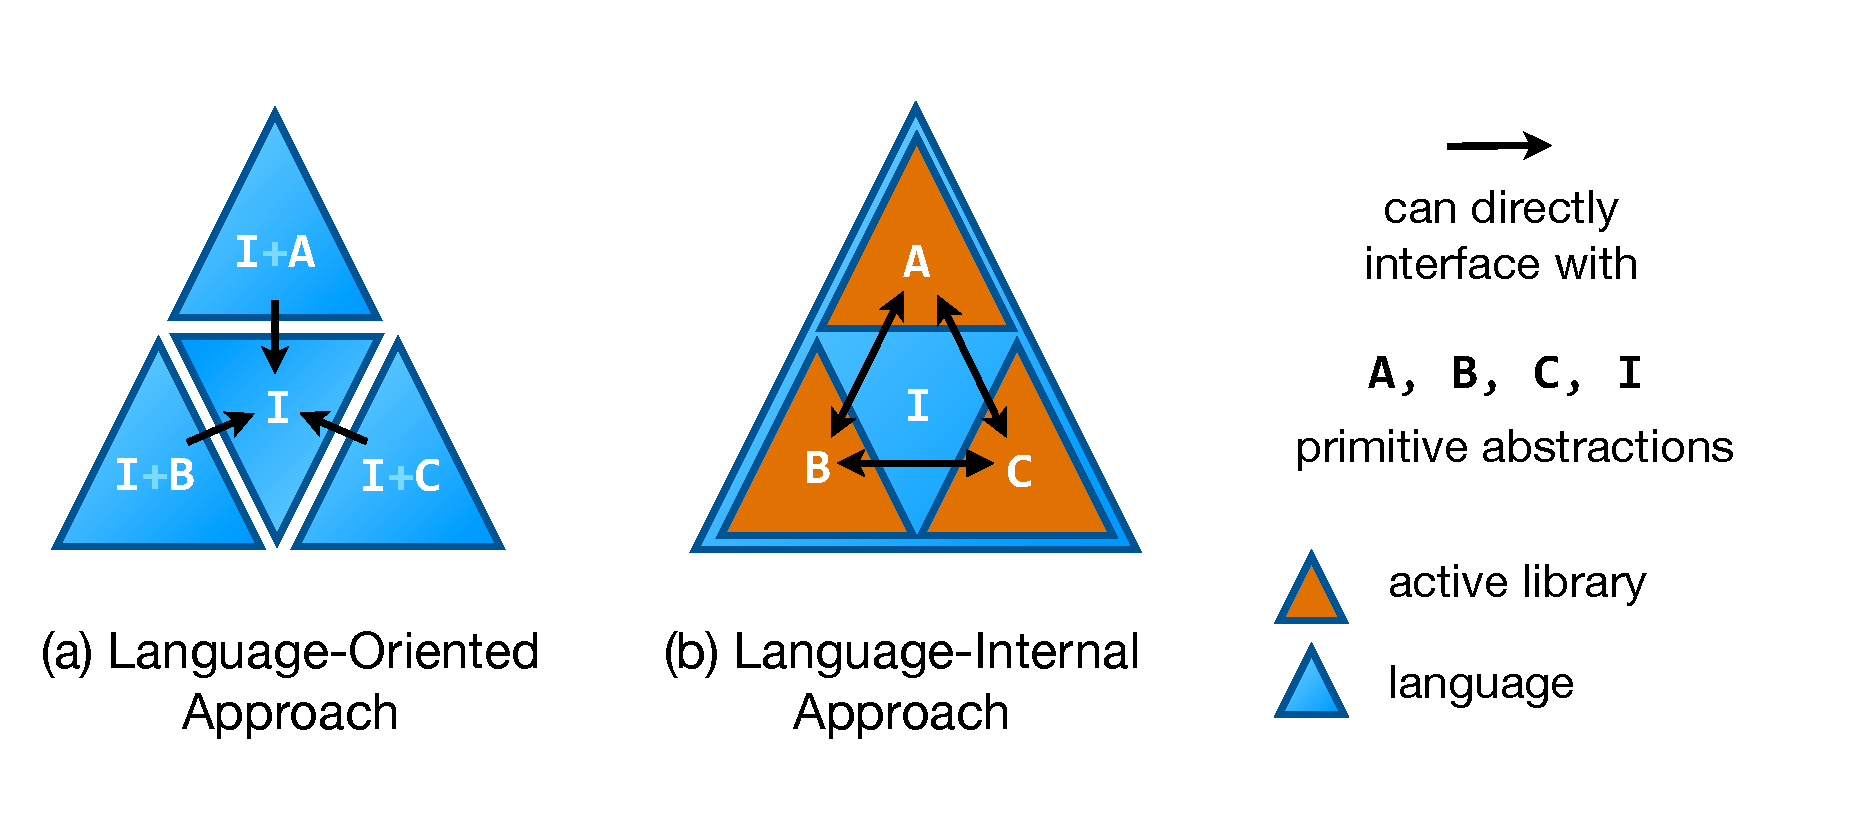
\includegraphics[scale=0.5]{approaches.pdf}
%\end{center}
%\vspace{-20px}
%\caption{\small (a) With a language-oriented approach, novel constructs are packaged into separate languages. Users can only safely and naturally call into languages consisting of common constructs (often only the common target language, such as C or Java bytecode). (b) With a language-internal extensibility approach, there is one system providing a common internal language, where additional primitive constructs that strictly strengthen its static guarantees or perform specialized code generation are specified and distributed within libraries. \label{approaches}}
%\end{figure*}

%As a result, domain-specific languages and new general-purpose abstractions alike have experienced relatively slow adoption in practice.
%
%Porting large codebases to new languages is difficult, and the dominant programming languages innovate slowly, so programming language.
%
%More specifically, such languages are neither \emph{internally extensible} because the language itself exposes only natural numbers and functions to its users, nor are they \emph{externally extensible} because no new behaviors can be added to the language's  implementation in a separate module from the one containing the initial implementation.

%This is the essence of a monolithic language implementation: it is impossible for anyone to modularly extend languages defined in this way. 

%An extensible programming language could address these problems by providing a language-integrated mechanism for introducing new type and operator constructors and implementing their associated static and dynamic semantics directly. 
%%Library developers need only consider which abstractions are most appropriate for their domain, without also considering whether these constructs can be exposed using abstractions appropriate to the domains of client code. Clients can simply import any necessary constructs when using a library that relies on them, preserving safety and ease-of-use without the use of  wrappers and glue code. We show this competing approach in Figure \ref{approaches}(b).
%%Researchers and domain experts thus gain the ability to distribute new ideas for evaluation to a broader development community without requiring the approval of maintainers of mainstream languages, large-scale porting of code or explicit interoperability layers. 
%But, as mentioned in Section \ref{language-integrated-approaches}, some significant challenges must be addressed before such a mechanism can be relied upon. The desire for expressiveness must be balanced against  concerns about maintaining various safety properties in the presence of arbitrary combinations of user-defined  extensions to the language's core semantics. The mechanism must ensure that desirable \emph{metatheoretic properties} (e.g. type safety, decidability) of the language are maintained by extensions. Because multiple independently developed extensions might be used within one program, the mechanism must further guarantee their \emph{non-interference}. These are the issues we seek to address in this work.

%When designing and implementing a new abstraction, experts typically begin by attempting to define new constructs in terms of existing language constructs.
%This approach is often effective because modern {general-purpose} abstraction mechanisms, like inductive datatypes and object systems, are highly expressive.  
%For example, the Delite framework leverages Scala's powerful general-purpose mechanisms to enable a number of useful \emph{embedded domain-specific languages} \cite{delite}.
%Unfortunately, there remain some situations of interest where general-purpose abstractions fall short. 
%For instance, it is difficult to adequately encode advanced type systems in terms of the simpler rules that govern general-purpose abstractions (e.g. reasoning about units of measure requires built-in language support in F\# \cite{conf/cefp/Kennedy09}). 
%Even if a full encoding is possible, it may not be useful if it is overly verbose or unnatural, or if the error messages are overly abstract. For example, regular expressions encoded using inductive datatypes are quite verbose, so most functional languages support them via strings, which is less safe. 
%Finally, general-purpose abstractions are implemented in a uniform manner, meaning domain-specific heuristics cannot be applied to eliminate overhead or perform optimizations, and implementations designed for typical application workloads may not be satisfactory in parts of a program where performance is a key criteria, such as when targeting heterogeneous hardware platforms (e.g. programmable GPUs) and distributed computing resources.
%
%% are at times impossible or impractical. In our example of adding products or sums to Godel's T, although Church encodings are possible \cite{pfpl}, they require a reasonable level of creativity\footnote{Anecdotally, Church encodings are among the more difficult-to-explain topics covered in our undergraduate programming languages course.}. Moreover, they will not offer the same static safety guarantees as a primitive encoding, they are more verbose and they will incur performance overhead by their use of closures rather than a more direct representation. This is not only a problem for simple languages like Godel's T. Several Haskell-based embedded DSLs have also needed to make significant compromises at times \cite{haskellDSLs}. {\color{red} examples? Scala?}
%
%%creating a new language. If this is not practical, the best one can attempt to do is encode the new types in terms of existing types (by a Church encoding, for example). This is generally unsatisfactory -- 
%
%%Languages implemented using these common patterns are central planning by a language designer or design committee. 
%
%Researchers or domain experts who run into situations like these, where more direct control over a language's semantics and implementation are needed, have little choice today but to realize new abstractions by creating a new language in some way. They might develop a new standalone language from scratch, modify an implementation of an existing language, or use tools like compiler generators, DSL frameworks and language workbenches \cite{fowler2010domain}. 
%%In our simple scenario, we may simply fork our implementation of Godel's T or even edit it directly (a pernicious technique for implementing a new language where the prior one is overwritten). 
%%In a more complex scenario, we may instead employ a tool like a compiler generator or DSL framework \cite{fowler2010domain} that can generate a standalone implementation from declarative specifications of language constructs. Some of these tools allow you to package and reuse these specifications (with the important caveat that not all combinations of constructs are valid and free of conflicts, an important modularity issue that we will return to several times in this paper).
%The increasing sophistication and ease-of-use of these tools have led to calls for a {\it language-oriented approach} to software development, where different components of an application are written in different specialized languages \cite{journals/stp/Ward94}. Indeed, a number of software ecosystems are now designed explicitly to support many different languages, both general-purpose and domain-specific, atop a common intermediate language. The Java virtual machine (JVM), the Common Language Infrastructure (CLI) and LLVM are prominent examples of such ecosystems.
%
%Unfortunately, this leads to a critical problem at language boundaries: a library's external interface must only use constructs that can reasonably be expressed in \emph{all possible client languages}. This discourages languages from including constructs that rely on statically-checked invariants stronger than those supported by their underlying implementation in the common intermediate language. At best, constructs like these can be exposed by generating a wrapper where run-time checks have been inserted to guarantee these invariants. This compromises both verifiability and performance. %Forrequires the development of an interoperability layer for every pair of DSLs. 
%Moreover, this approach exposes the internals of an implementation to clients, making the abstraction awkward to work with and causing code breakage when implementation details change. This defeats a primary purpose of high-level programming languages: hiding low-level details from clients of an abstraction. We diagram this fundamental \emph{interoperability problem} in Figure \ref{approaches}(a). 
%%As an example, F\#'s type system prevents \lstinline{null} values from occurring within data structures, but because it's type system is not available when calling into F\# code from another language, like C\#, run-time null checks must still be included in the implementation.
%%\begin{figure*}[t]
%%\vspace{-15px}
%%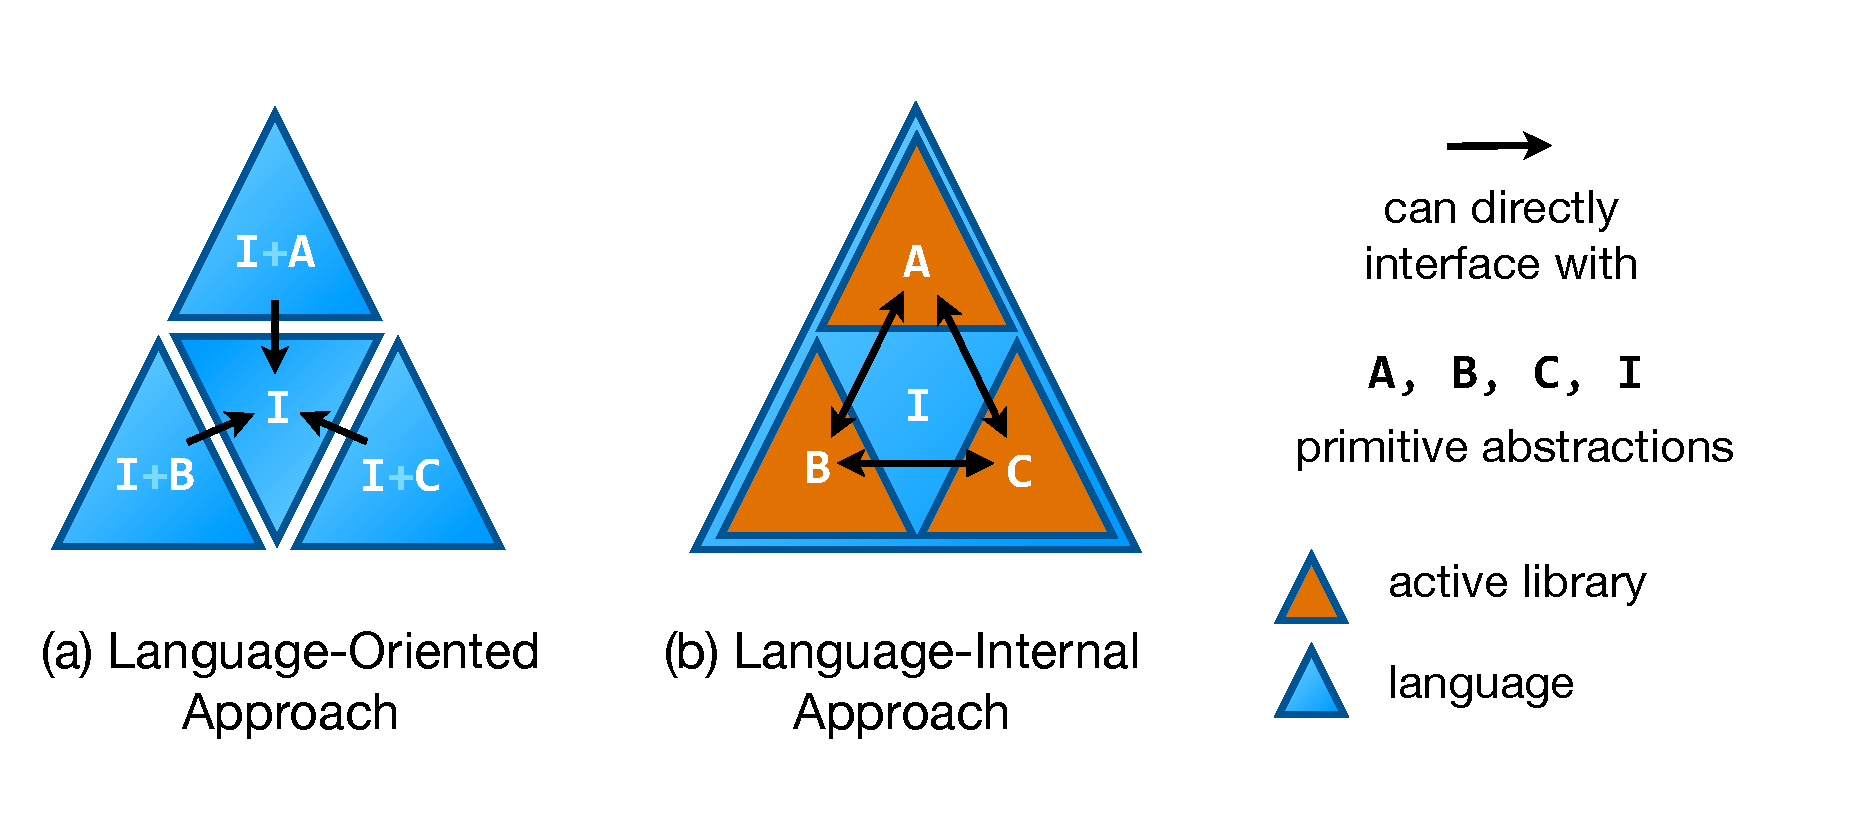
\includegraphics[scale=0.415]{approaches.pdf}
%%\caption{(a) With the language-oriented approach, different primitive abstractions are packaged into separate languages that extend and target a common intermediate language (e.g. JVM bytecode). Users can only interface with libraries written in another language via the constructs in the common language, causing \emph{interoperability problems}. (b) With the language-internal approach, the semantics of new abstractions (i.e. the logic that governs typechecking and translation to a fixed {internal language}, here labeled \texttt{I}) can be implemented directly within so-called \emph{active libraries}. Clients can import and use these abstractions directly whenever needed.}
%%\label{approaches}
%%\end{figure*}
%
%%As a result, domain-specific languages and new general-purpose abstractions alike have experienced relatively slow adoption in practice.
%%
%%Porting large codebases to new languages is difficult, and the dominant programming languages innovate slowly, so programming language.
%%
%%More specifically, such languages are neither \emph{internally extensible} because the language itself exposes only natural numbers and functions to its users, nor are they \emph{externally extensible} because no new behaviors can be added to the language's  implementation in a separate module from the one containing the initial implementation.
%
%%This is the essence of a monolithic language implementation: it is impossible for anyone to modularly extend languages defined in this way. 
%
%%Programming languages are typically designed around a monolithic collection of primitive type families and operators. Consider, as a simple example, Godel's T \cite{pfpl}, a typed lambda calculus with recursion on primitive natural numbers\todo{add statics to Appendix A}. Although a language designer may casually speak of ``extending Godel's T with primitive product and sum types'', adding these type families and associated operators to this kind of language from within is impossible. That is, Godel's T is not \emph{internally extensible}.
%
%\emph{Internally-extensible programming languages} promise to avoid these problems by providing researchers and domain experts with a mechanism for implementing the semantics of new primitive constructs directly within libraries.
%%Developers of libraries need only determine whether they are appropriate for their domain, without also considering whether these constructs can be exposed in terms of abstractions appropriate to client code. 
%As a result, clients can granularly import any necessary primitive constructs when using code that relies on them, and thereby achieve full safety, ease-of-use and performance. Providers of components thus need only consider whether primitives that they use are appropriate for their domain, without also considering whether their code might be used in a context where these primitives are not otherwise appropriate. Libraries containing logic that is invoked at compile-time, as extension logic would be, have been called \emph{active libraries} \cite{activelibraries}. We adopt this terminology and diagram this competing approach in Figure \ref{approaches}(b).
%
%%Researchers and domain experts thus gain the ability to distribute new ideas for evaluation to a broader development community without requiring the approval of maintainers of mainstream languages, large-scale porting of code or explicit interoperability layers. 
%
%For a language-internal extension mechanism to be feasible, however, it must achieve expressiveness while also ensuring that extensions cannot compromise the safety properties of the language and its tools, nor interfere with one another. That is, extensions cannot simply be permitted to add arbitrary logic to the type system or compiler, because this would make it possible to break  type safety, decidability or adequacy theorems that are critical to the operation of the language, the compiler or other extensions. We review some previous attempts at language extensibility, and highlight how they do not adequately achieve both safety and expressiveness, in Section \ref{related-work}.
%%{\color{red} transition here} Correctness properties of an extension itself should be modularly verifiable, so that its users can rely on it for verifying and compiling their own code. The mechanism must also ensure that desirable metatheoretic properties and global safety guarantees of the language cannot be weakened by extensions. And with multiple independently-developed extensions used at once, the mechanism must further guarantee that they cannot interfere with one another. 
%
%In this paper, we introduce a language-internal extensibility mechanism called \emph{active typechecking and translation} (AT\&T) that allows developers to introduce and implement the logic governing new primitive type and operator families from within libraries. 
%We argue that this can be accomplished by enriching the type-level language, rather than introducing a separate metalanguage into the system. 
%To make this proposal concrete, we begin by introducing a simple core calculus, called \atlam~(for the ``actively-typed lambda calculus''), in Section \ref{atlam}. 
%This calculus uses type-level computation of higher kind, along with techniques borrowed from the typed compilation literature and a form of type abstraction that ensures that the implementation details of an extension are not externally visible to guarantee the safety of the language, the decidability of typechecking and compilation and non-interference of extensions, as we outline in Section \ref{safety}.
%In Section \ref{examples}, we suggest that despite these constraints, this mechanism is expressive enough to admit, within libraries, a number of general-purpose and domain-specific abstractions that normally require built-in language support. 
%
%Our core calculus uses a uniform abstract syntax for primitive operators to simplify our presentation and analysis, but this syntax is too verbose to be practical. Thus, we begin this section by showing how a key design choice made in the calculus -- to associate operators with type families, forming what we call \emph{active type families} -- supports a novel type-directed desugaring mechanism that permits the use of conventional concrete syntax for language extensions. 

% Our choice of a simply-typed, simply-kinded calculus where expressions are given meaning by translation to a simply-typed internal language appears to occupy a ``sweet spot'' in the design space, and relates closely to how simply-typed functional languages like  ML and Haskell are specified and implemented today. In Section \ref{design}, we briefly discuss other points in the design space of actively-typed languages and describe the sorts of abstractions that the mechanism as we have introduced it is not capable of expressing, suggesting several directions for future research. We conclude with a discussion of related work in Section \ref{related-work}.
%dependently-typed and object-oriented type-level languages, as well as the constraints governing the design of the internal language.  
%We will also note how object-oriented techniques may also be suit, because of a fundamental connection to the \emph{expression problem} \cite{expression-problem}.

%specify new typechecking rules and translation logic from within libraries. The AT\&T mechanism utilizes type-level computation of higher kind and integrates typed compilation techniques into the language to provide strong safety guarantees, while remaining straightforward and expressive.

%AT\&T is general with respect to many choices about the type-level language, the typed internal language and syntax. Choices along these dimensions can affect both expressiveness and ease-of-use. We will begin in Sec. 2 by introducing a minimal system called $@\lambda$ (the ``actively-typed lambda calculus'') that distills the essence of the mechanism in a simply-typed, simply-kinded setting. This will allow us to fully and concisely formalize the language and compiler and give several key safety theorems. We will then continue in Sec. 3 by discussing variants of this mechanism based on other basic paradigms, considering dependently-typed functional languages and object-oriented languages, discussing trade-offs between expressivity and safety when doing so. We have developed a simple prototype called Ace and have used it to develop a number of full-scale language extensions as libraries. We will briefly discuss this language and these extensions in Sec. 4.

%We note at the outset that AT\&T focuses on extending the static semantics of languages with fixed, though flexible, syntax. Language-internal syntax extension mechanisms have been developed in the past (e.g. SugarJ \cite{sugarj}) but they have also suffered from safety problems because grammar composition is not always safe when done in an  unconstrained manner. Constrained approaches that provide stronger safety guarantees have recently been outlined (e.g. Wyvern \cite{globaldsl13}) but we will leave integration of syntax extensions with semantic extensions as future work.
%\section{From Extensible Compilers to Extensible Languages}\label{evolution}
%\begin{figure}[t]
%\small
%$$\begin{array}{rccl}	
%\textbf{programs} & \rho & ::= & \pfam{\familyDf}{\progsort}  \\
% & & \pipe &  \pdef{t}{\kappa}{\tau}{\progsort} \pipe e\\
%\text{primitive ops}		&	\theta	&	::= &	\tops{op}{\kappaidx}{i}{a}{\tau} \pipe 
%												\topp{\theta}{\theta}\\
%\\
%\textbf{external terms} 				&	e	&	::=	&	\evar{x} \pipe 
%														\elam{\evar{x}}{\tau}{e} \pipe 
%														\eop{Fam}{op}{
%															\taui
%														}{
%  												    		\splat{e}{1}{n}
%														} \\
%									& 		&		& 	\\
%							
%\hspace{-5pt}\textbf{type-level terms} 	& \tau 	& ::= 	& 	\tvar{t} \pipe 
%														\tlam{t}{\kappa}{\tau} \pipe 
%														\tapp{\tau_1}{\tau_2}\pipe
%														\iintlit \pipe \iop{\tau_1}{\tau_2} \pipe \tstr{str} \\
%									    & &  \pipe & 
%														\tnil{\kappa} \pipe \tcons{\tau_1}{\tau_2} \pipe 
%									                     \tfold{\tau_1}{\tau_2}{h}{t}{r}{\tau_3}
%														\\
%												
%	 			& 		& \pipe	& 	 \tunit \pipe 
%														\tpair{\tau_{1}}{\tau_{2}} \pipe 
%														\tfst{\tau} \pipe 
%														\tsnd{\tau} 
%														\\
%\text{equality}  & & \pipe & 					\tifeq{\tau_{1}}{\tau_{2}}{\kappa}{\tau_{3}}{\tau_{4}} 
%														\\														
%
%\text{types} 						& 		& \pipe	& 	\ttypestd \\
% & & \pipe &  \tfamcase{\tau}{Tycon}{x}{\tau_1}{\tau_2}\\
%						%				& & \pipe & \tfamcase{\tau}{Fam}{x}{\tau_1}{\tau_2}\\
%																								
%\text{denotations} 				& 		 & 	\pipe	&	\tden{\tauiterm}{\tautype} \pipe \terr \\
% & & \pipe &  \tdencase{\tau}{x}{t}{\tau_1}{\tau_2}\\
% %& & \pipe & 
%%														\tdencase{\tau}{y}{x}{\tau_1}{\tau_2}
%%														 \\
%
%\text{reified IL}		&		&	\pipe	&	\titerm{\iota} \pipe \titype{\sigma} \\
%
%												\\
%\textbf{kinds} 					& \kappa	&	::=	&	\karrow{\kappa_1}{\kappa_2} \pipe \klist{\kappa} \pipe \dint \pipe
%											    \kstr \pipe
%												\kunit \pipe 
%												\kpair{\kappa_{1}}{\kappa_{2}} \\
%	& & \pipe &  
%												\kTypeBlur \pipe \kDen \pipe 
%												\kIType \pipe \kITerm
%												\\
%\\												
%%\textbf{ops signature}			& \Theta	&	::=	&	\kOpEmpty \pipe \kOp{\Theta}{op}{\kappai}\\
%%											 							&		&		&	\\
%\textbf{internal terms} 				& 	\iota	&	::=	&	\evar{x} \pipe 
%												\ilam{\evar{x}}{\sigma}{\iota} \pipe 
%												\iapp{\iota_{1}}{\iota_{2}} \pipe
%												\ifix{\evar{f}}{\sigma}{\iota} \\
%									& & \pipe & 
%												\ipair{\iota_{1}}{\iota_{2}} \pipe 
%												\ifst{\iota} \pipe
%												\isnd{\iota}  
%												\\
%							& 		& 	\pipe	& 
%												\iintlit \pipe \iop{\iota_{1}}{\iota_{2}} \pipe \iIfEq{\iota_{1}}{\iota_{2}}{\dint}{\iota_{3}}{\iota_{4}}  
%												\\
% &  & \pipe & \tvalof{\tau_1}{\tau_2} \pipe \iup{\tau} \\
%%\text{deabstracted}& \iota & ::= & \mathcal{G}[\iota, \sigma]\\
%\textbf{internal types}			&	\sigma	&	::=	&    \darrow{\sigma_1}{\sigma_2} \pipe
%												\dint \pipe
%												\dpair{\sigma_1}{\sigma_2} \pipe
%												\trepof{\tau} \pipe \dup{\tau}\\
%\end{array}$$
%%\vspace{-10pt}
%\caption{\small Syntax of \atlam. Variables $x$ are used in expressions and internal terms and are distinct from type-level variables, $\tvar{t}$. Names $\fvar{Fam}$ are type family names (we assume that globally unique type family names can be generated by some external mechanism) and $\opvar{op}$ are operator family names. $\tstr{str}$ denotes string literals, $\iintlit$ denotes integer literals and $\oplus$ stands for binary operations over integers. %The productions related to the internal language are written using generators $\mathcal{G}$ and $\mathcal{S}$ to avoid duplicating the syntax of common terms.
%\label{grammar}}
%\end{figure}
%\begin{figure}[t]
%\small
%\begin{flalign}
%\label{natfam}&\family{Nat}{\kunit}{\\
%\label{z}&\quad\tops{z}{\kunit}{i}{a}{
%	\tapp{\tapp{\tvar{empty}}{\tvar{a}}}{
%		\tden{\titerm{0}}{\ttype{Nat}{\tunit}}
%	}};\\
%\label{s}&\quad\tops{s}{\kunit}{i}{a}{
%	\tapp{
%		\tapp{\tvar{pop\_final}}{\tvar{a}}}{\tlam{x}{\kITerm}{\tlam{t}{\kTypeBlur}{
%			\\
%			&\quad\quad\tapp{\tapp{\tapp{\tvar{check\_type}}{\tvar{t}}}{\ttype{Nat}{\tunit}}}{
%				\tden{\titerm{\iup{\tvar{x}}+1}}{\ttype{Nat}{\tunit}}
%			}
%		}}
%		}
%	};\\
%\label{rec}&\quad\tops{rec}{\kunit}{i}{a}{
%	\tapp{\tapp{\tvar{pop}}{\tvar{a}}}{\tlam{x1}{\kITerm}{\tlam{t1}{\kTypeBlur}{\tlam{a}{\klist{\kDen}}{\\
%	&\quad\quad\tapp{\tapp{\tvar{pop}}{\tvar{a}}}{\tlam{x2}{\kITerm}{\tlam{t2}{\kTypeBlur}{\tlam{a}{\klist{\kDen}}{\\
%	&\quad\quad \tapp{\tapp{\tvar{pop\_final}}{\tvar{a}}}{\tlam{x3}{\kITerm}{\tlam{t3}{\kTypeBlur}{\\
%	&\quad\quad \tapp{\tapp{\tapp{\tvar{check\_type}}{\tvar{t1}}}{\ttype{Nat}{\tunit}}}{(\\
%	&\quad\quad \tapp{\tapp{\tapp{\tvar{check\_type}}{\tvar{t3}}}{\ttype{Arrow}{(\ttype{Nat}{\tunit},\ttype{Arrow}{(\tvar{t2},\tvar{t2})})}}}{\\
%		\label{fix}&\quad\quad \tden{\titerm{\iapp{(\ifix{f}{\darrow{\dint}{\trepof{\tvar{t2}}}}{\ilam{x}{\dint}{\\
%		\label{lastop}&\quad\quad\quad \iIfEq{x}{0}{\dint}{\iup{\tvar{x2}}}{\iapp{\iapp{\iup{\tvar{x3}}}{(x-1)}}{(\iapp{f}{(x-1)})}}}})}{\iup{\tvar{x1}}}}}{\tvar{t2}}
%	)}}
%	}}}}}}}}}}}}
%\\
%&}{XXX}{i}{\titype{\dint}};\\
%\label{nattype}&\pdef{nat}{\kTypeBlur}{\ttype{Nat}{\tunit}}{\\
%\label{plus}&(\elam{plus}{\ttype{Arrow}{(\tvar{nat}, \ttype{Arrow}{(\tvar{nat}, \tvar{nat}))}}}{
%	\elam{two}{\tvar{nat}}{\\
%\label{ap}	&\quad\quad \eopapp{\eopapp{plus}{two}}{two}}})
%}\\
%\label{add}&\quad (\elam{x}{\tvar{nat}}{\elam{y}{\tvar{nat}}{
%	\eop{Nat}{rec}{\tunit}{x; y; \elam{p}{\tvar{nat}}{\elam{r}{\tvar{nat}}{
%	\eop{Nat}{s}{\tunit}{r}
%	}}}}})\\
%\label{two}&\quad  \eop{Nat}{s}{\tunit}{\eop{Nat}{s}{\tunit}{\eop{Nat}{z}{\tunit}{ }}}
%%{\\&\elet{two}{\tvar{nat}}{\eop{Nat}{s}{\tunit}{\eop{Nat}{s}{\tunit}{\eop{Nat}{z}{\tunit}{ }}}}{\eapp{\eapp{plus}{two}}{two}}}
%%}
%%\elam{x}{\tvar{nat}}{\elam{y}{\tvar{nat}}{\\
%	%&\quad \eop{Nat}{rec}{\tunit}{x; y; \elam{p}{\tvar{nat}}{\elam{r}{\tvar{nat}}{
%	%\eop{Nat}{s}{\tunit}{r}
%	%}}}}
%\end{flalign}
%\caption{G\"odel's T in \atlam, used to calculate 2+2. Helper functions for working with lists ($\tvar{empty}$, $\tvar{pop}$, $\tvar{pop\_final}$) and types ($\tvar{check\_type}$),  described below, are given in the appendix. We will refer to this program as $\rho_{\text{nat}}$ in the text.}
%\label{example}
%\end{figure}
%
%To understand the genesis of our internal extension mechanism, it is helpful to begin by considering why most implementations of programming languages cannot even be  externally extended. 
%Let us consider, as a simple example, an implementation of G\"odel's T, a typed lambda calculus with recursion on primitive natural numbers (see Appendix). 
%A compiler for this language written using a functional language will invariably represent the primitive type families and operators using {closed} inductive datatypes. 
%For example, a simple implementation in Standard ML may be based around these datatypes:
%\begin{lstlisting}
%  datatype Type = Nat | Arrow of Type * Type
%  datatype Exp = Var of var 
%               | Lam of var * Type * Exp | Ap of Exp * Exp 
%               | Z | S of Exp | Natrec of Exp * Exp * Exp
%\end{lstlisting}
%
%The logic governing typechecking and translation to a suitable intermediate language (for subsequent optimization and compilation by some back-end) will proceed by exhaustive case analysis over the constructors of \lstinline{Exp}.
%
%In an object-oriented implementation of Godel's T, we might instead encode types and operators as subclasses of abstract classes \lstinline{Type} and \lstinline{Exp}. Typechecking and translation will proceed by the ubiquitous \emph{visitor pattern}  by dispatching against a fixed collection of {known} subclasses of \lstinline{Exp}. 
%
%In either case, we encounter the same basic issue: there is no way to modularly add new primitive type families and operators and implement their associated typechecking and translation logic. 
%%This issue is related to the widely-discussed \emph{expression problem} (in a restricted sense -- we do not consider adding new functions beyond typechecking and translation here, only adding logic to these) \cite{wadler-expression}.
%
%A number of language mechanisms have been proposed that allow new cases to be added to datatypes and the functions that operate over them in a modular manner. 
%In functional languages, we might use \emph{open datatypes}. For example, if we wish to extend G\"odel's T with product types and we have written our compiler in a language supporting open inductive datatypes, it might be possible to add new cases like this: 
%\begin{lstlisting}
%  newcase Prod of Type * Type extends Type
%  newcase Pair of Exp * Exp extends Exp    (* Intro *)
%  newcase PrL of Exp extends Exp           (* Elim Left *)
%  newcase PrR of Exp extends Exp           (* Elim Right *)
%\end{lstlisting}
%
%The logic for functionality like typechecking and translation could then be implemented for only these new cases. For example, the \lstinline{typeof} function that assigns a type to an expression could be extended like so:
%\begin{lstlisting}
%  typeof PrL(e) = case typeof e of 
%      Prod(t1, _) => t1 
%    | _ => raise TypeError("<appropriate error message>")
%\end{lstlisting}
%
%If we allowed users to define new modules containing definitions like these and link them into our compiler, we will have succeeded in creating an externally-extensible compiler, albeit one where safety is not guaranteed (we will return to this point shortly). We have not, however, created an extensible programming language, for two reasons. First, compiler extensions are distributed and activated separately from libraries, so dependencies become more difficult to manage. Second, other compilers for the same language will not necessarily support the same extensions. 
%If our newly-introduced constructs are exposed at a library's  interface boundary, clients using different compilers face the same problems with interoperability that those using different languages face. That is, {extending a language by extending a single compiler for it is morally equivalent to creating a new language}. Several prominent language ecosystems today are in a state where a prominent compiler has introduced or enabled the introduction of extensions that many libraries have come to rely on, including the Glasgow Haskell Compiler, SML/NJ and the GNU compilers for C and C++.
%
%A more appropriate and useful place for extensions like this is directly within libraries, alongside abstractions that can be adequately implemented in terms of existing primitive abstractions. To enable this, the language must allow for the introduction new primitive type families, like \lstinline{Prod}, operators, like \lstinline{Pair}, \lstinline{PrL} and \lstinline{PrR}, and associated typechecking and translation logic. When encountering these new operators in expressions, the compiler must effectively  hand control over typechecking and translation to the appropriate user-defined logic. Because this mechanism is {language-internal}, all compilers must support it to satisfy the language specification.
%
%Statically-typed languages typically make a distinction between \emph{expressions}, which describe run-time computations, and type-level constructs like types, type aliases and datatype declarations. The design described above suggests we may now need to add another layer to our language, an {extension language}, where extensions can be declared and implemented. In fact, we will show that \textbf{the most natural place for type system extensions is within the type-level language}. The intuition is that extensions to a statically-typed language's semantics will need to manipulate types as values at compile-time. Many languages already allow users to write type-level functions for various reasons, effectively supporting this notion of types as values at compile-time (see Sec. \ref{related-work} for examples). The type-level language is often constrained by its own type system (where the types of type-level values are called \emph{kinds} for clarity) that prevents type-level functions from causing problems during compilation. This is precisely the structure that a distinct extension layer would have, and so it is quite natural to unify the two, as we will show in this work.
%
%\section{\atlam}\label{atlam}
%In this section, we will develop a core calculus, called @$\lambda$ for the ``actively-typed lambda calculus'', by way of a semantics and a simple example, and discuss how it addresses the safety concerns that arise. 
%\subsection{Overview}
%The grammar of \atlam~is shown in Figure \ref{grammar}. 
%A program, $\rho$, consists of a series of declarations followed by an expression. Declarations can be either bindings of type-level terms to type-level variables using \textsf{def} or a primitive type family declared using \textsf{family}, which can contain implementations of one or more operator families, $\theta$. Expressions, $e$, can be either variables, lambdas, or applications of operators.
%%, and are ultimately given meaning by translation to a typed internal language, with terms $\iota$ and types $\sigma$. 
%%This language has been chosen, for simplicity, to be a variant of Plotkin's PCF with primitive integers and products, but in practice would include other constructs consistent with its role as a high-level intermediate language.
%
%The language is structured as a simply-typed lambda calculus with simply-kinded type-level computation. Kinds, $\kappa$, classify type-level terms, $\tau$. 
%Types are type-level values of kind $\star$ (following System $F_{\omega}$) and classify expressions. The type-level language also includes other kinds of terms: type-level functions, lists (required by our mechanism), integers, strings and products for the sake of our examples (see Sec. \ref{safety} for a discussion on other acceptable kinds of type-level data) and constructs for developing extensions -- denotations and reified internal terms and types -- which we will discuss in the sections below. 
%
%All expressions are given meaning by translation to a typed internal language. This language has been chosen, for simplicity, to be a variant of Plotkin's PCF with primitive integers and products, but in practice would include other constructs consistent with its role as a high-level intermediate language. The grammar of internal terms, $\iota$, and internal types, $\sigma$, also includes special forms containing type-level terms; these are used for developing extensions and during compilation and will be erased before compilation ends.
%\subsection{Example: G\"odel's T as an Active Type Family}
%To make our explanation of each of the constructs in the calculus concrete, we will work through an example showing how to introduce primitive natural numbers with bounded recursion in the style of G\"odel's T \cite{pfpl}. These will be implemented internally as integers (that is, internal terms of internal type $\dint$). Figure \ref{example} shows how to define the indexed type family $\fvar{Nat}$. This family contains only one type, written $\ttype{Nat}{\tunit}$, which we alias on line \ref{nattype} by defining the type-level variable $\tvar{nat}$. We define the typechecking and translation logic for the operators associated with this family (\opvar{z}, \opvar{s} and \opvar{rec}) on lines \ref{z}-\ref{lastop} and use these to define a $plus$ function on line \ref{add} and compute 2+2. We will refer back to this figure as we describe each construct below.
%
%\subsection{Indexed Type Families and Types}\label{families}
%The syntactic form $\familyDf$ declares a new primitive type family named $\fvar{Fam}$ indexed by type-level values of kind $\kappaidx$ with representation schema $\tvar{i}.\taurep$ and operators $\theta$. The purpose of the representation schema and of associating of operators directly with types will be explained below. 
%
%Declaring a type family in this way is a language-internal analog to adding a new constructor to the compiler-internal datatype \lstinline{Type}, as suggested in Sec. \ref{evolution}. 
%The index represents the data associated with this constructor. A type (that is, a type-level term of kind $\kTypeBlur$) is constructed by naming a family in scope and providing a type-level term of the appropriate kind as an index. A base type like $\tvar{nat}$ can be thought of as being the only type in the family $\fvar{Nat}$ trivially indexed by the unit value, of kind $\kunit$, while families like $\fvar{Ntuple}$ might be indexed by a list of types, having kind $\klist{\kTypeBlur}$. 
% For example, $\ttype{Ntuple}{\tcons{\tvar{nat}}{\tcons{\tvar{nat}}{\tnil{\kTypeBlur}}}}$ might be the type of a pair of natural numbers. Given a type, its family can be \textsf{case} analyzed to extract the value of its index. It is important that type equality be decidable, so only kinds for which equivalence coincides with syntactic equality can be used as type family indices. The main  consequence of this restriction is that indices cannot contain type-level functions.
%
%\subsection{Representations and Representation Schemas}
%As we will discuss further below, it is important that all expressions classified by a type compile to consistently-typed internal terms. For this reason, we require that every type have a single internal type associated with it, called its \emph{representation}. This is computed by substituting the type index for the bound variable $\tvar{i}$ in the term $\taurep$, called the \emph{representation schema} of the type family, and evaluating to a value representing an internal type. Internal types, $\sigma$, are reified as type-level terms of kind $\kIType$ using the introductory form $\titype{\sigma}$.
%
%\subsection{Indexed Operator Families and Denotations}\label{operators}
%Type families are also equiped with a collection of primitive operator families. An operator family named $\opvar{op}$ is declared using the form $\tops{op}{\kappaidx}{i}{a}{\tauop}$. Like type families, operator families are indexed by values of some kind, $\kappaidx$, but because operators are not first-class type-level values in our calculus, there are no equality restrictions. In the example in Fig. \ref{example}, all the operators are trivially indexed by the kind $\kunit$, so each family only contains one operator. However, a type family like $\fvar{Ntuple}$ would be equipped with a family of projection operators, $\opvar{pr}$, indexed by a position (e.g. an integer in our calculus). A family implementing record types or object types might have a similar operator indexed by a type-level string representing the field being accessed (see Sec. \ref{examples}).
%
%To apply an operator, the grammar provides a uniform form of expression: $\eop{Fam}{op}{\tauidx}{e_1; \ldots; e_n}$, where $n \geq 0$. The typechecking and translation of an expression of this form is controlled by the term $\tauop$ in the operator's declaration. This term must evaluate to a \emph{denotation}, which is a type-level value of kind $\kDen$, when given the operator index, $\tauidx$, and a list constructed from the denotations recursively assigned to each argument, $e_1$ through $e_n$. 
%
%There are two forms of denotations that an expression can be assigned. A \emph{valid denotation} has the form $\tden{\tauiterm}{\tautype}$, where $\tauiterm$ is the \emph{translation} of the expression to an internal term and $\tautype$ is the type it has been assigned. Internal terms are represented as type-level terms using the form $\titerm{\iota}$, and have kind $\kITerm$ (similar to $\kIType$). %It is important to note that there are no elimination form for reified terms or types.
%%(indeed, in \atlam, terms are never  syntactically analyzed directly by extensions, unlike macro systems and other forms of term rewriting; see Sec. \ref{related-work})
%If a type error is detected by an operator, the \emph{error denotation}, $\terr$, is returned instead of a valid denotation. In a practical implementation, a specialized error message and other diagnostic information would be provided when returning $\terr$, but we omit such details for simplicity. Terms of kind $\kDen$ can be \textsf{case} analyzed to determine if they are valid or errors, and if valid, to extract the translation and type.
%
%In the example in Fig. \ref{example}, the operator $\opvar{z}$ checks that no arguments were passed in using the simple helper function $\tvar{empty}$. If so, it returns a valid denotation by pairing the translation $\titerm{0}$ with the type $\ttype{Nat}{\tunit}$, as expected\footnote{Actually, there is no theoretical barrier to a different ``zero'' being used!}. If an argument was provided, the helper function returns $\terr$. The successor operator, $\opvar{s}$, takes one argument, so it pops a denotation off the argument list, making sure there are no more, and binds its translation and type to $\tvar{x}$ and $\tvar{t}$ respectively, all using the helper function $\tvar{pop\_final}$. It then checks that the argument's type is also $\ttype{Nat}{\tunit}$, returning a denotation pairing the translation $\titerm{\iup{\tvar{x}} + 1}$ with the type $\ttype{Nat}{\tunit}$ if so. The form $\iup{\tau}$ is used to ``un-reify'' reified internal terms, of kind $\kITerm$ (thus serving as the left-inverse of $\titerm{\iota}$). In this case, $\tvar{x}$ is a type-level variable of kind $\kITerm$ representing the translation of the argument to the successor operator, so we simply need to add one to it. Because we have checked that the denotation's type was $\ttype{Nat}{\tunit}$, and the representation schema will guarantee that expressions of this type always translate to integers, we know that it is safe to do so. If any of these steps fail, the various helper functions we use simply return $\terr$ (in practice, it would be prudent to equip each failure condition with a different error message). Compilation will also fail if we accidentally violate the representation schema, as we will see in Sec. \ref{repcon}.
%
%% The operator index, $\tauidx$, and . 
%
%\subsection{Functions, Variables and Arrow Types}
%
%The recursor operator, $\opvar{rec}$, proceeds similarly, extracting the translations and types of each of its three arguments. Of note, however, is how it handles the third argument, which binds two variables (the predecessor and the result of recursing on it). In \atlam, the built-in $\lambda$ operator serves as the sole mechanism for introducing bound variables. In most calculi, lambda terms have types of the form $\tau_1 \rightarrow \tau_2$. In \atlam, $\rightarrow$ corresponds to the built-in type family, $\fvar{Arrow}$. This family is indexed by a pair of types, $\kpair{\kTypeBlur}{\kTypeBlur}$, and is always in scope. Its representation schema simply maps to the corresponding internal arrow type, $\tvar{i}.\titype{\darrow{\trepof{\tfst{\tvar{i}}}}{\trepof{\tsnd{\tvar{i}}}}}$. The special form $\trepof{\tau}$ is used to refer, abstractly, to the representation of the type $\tau$ (we also see this used on line \ref{fix}). Although the $\lambda$ operator is built-in, because it needs to bind variables, application is just an operator associated with the $\fvar{Arrow}$ family, $\opvar{ap}$, as is seen on line \ref{ap}. The details are straightforward and given in the appendix.
%
%\subsection{Compilation}
%\begin{figure}[t]
%\small
%\begin{mathpar}
%\inferrule{
%	\overbrace{\progOK{\emptyctx}{\fvalCtx_0}{\rho}}^{\text{\normalsize Kind Checking}}\\
%	\overbrace{\pcompiles{\fvalCtx_0}{\rho}{\iota}}^{\text{\normalsize Active Typechecking and Translation}}
%}{
%	\ptcc{\rho}{\iota}
%}
%\end{mathpar}
%\caption{\small Central Compilation Judgement of \atlam.}
%\label{ccj}
%\end{figure}
%The \emph{central compilation judgement}, shown in Figure \ref{ccj}, captures the two phases of compilation: kind checking and active typechecking and translation. 
%The first phase ensures that all type-level terms in the program are well-kinded and that all expressions and internal terms are closed. The kinding rules for programs are given in Figure \ref{kindprog}, and they rely on the kinding rules for type-level terms given in Figure \ref{tlkind}. These rules use contexts $\Sigma$ and $\Theta$ to track family and operator signatures, but beyond that, the rules are largely consistent with those of a simply-typed lambda calculus shifted into the type-level, with the addition of the handful of special forms constrained as described in the previous sections. The reader is encouraged to verify that the example in Fig. \ref{example} is well-kinded. 
%% As we will see, the kind checking phase ensures that many kinds of errors are ruled out and that this process will not ``get stuck'' (see Sec. \ref{safety}). The evaluation semantics for type-level terms are given in Fig. \ref{tleval}.
%\begin{figure}[t]
%\small
%$\fbox{\inferrule{}{\progOKX{\progsort}}}$
%~~~$\tvarCtx ::= \emptyctx \pipe \tvarCtxX{t}{\kappa}$~~~
%$\fCtx ::= \Sigma_0	 \pipe \fvalCtxX$
%\begin{mathpar}
%\inferrule[family-kinding]{
%	\fvar{Fam} \notin \text{dom}(\fvalCtx)\\
%	\kEq{\kappaidx}\\
%	\opType{\tvarCtx}{\fvalCtxX}{\theta}{\Theta}\\\\
%	\tKind{\tvarCtx, \tvar{i}:{\kappaidx}}{\fvalCtxX}{\tau}{\kIType}\\
%	\progOK{\tvarCtx}{\fvalCtxX}{\rho}
%}{
%	\progOKX{\pfam{\familyDf}{\rho}}
%}
%
%\inferrule[def-kinding]{
%	\tKindX{\tau}{\kappa}\\
%	\progOK{\tvarCtxX{t}{\kappa}}{\fvalCtx}{\rho}
%}{
%	\progOKX{\pdef{t}{\kappa}{\tau}{\rho}}
%}
%
%\inferrule[exp-kinding]{
%	\exprOK{\tvarCtx}{\emptyctx}{\fvalCtx}{e}
%}{
%	\progOKX{e}
%}
%\end{mathpar}
%$\fbox{$\tKindX{\theta}{\Theta}$}$
%~~~$\Theta ::= \kOpS{op}{\kappaidx} \pipe \Theta, \Theta$~~~
%\begin{mathpar}
%\inferrule[op-kinding]{
%	\tKind{\tvarCtx, \tOfKind{\tvar{i}}{\kappai}, \tOfKind{\tvar{a}}{\klist{\kDen}}}{\fvalCtx}{\tau}{\kDen}
%}{
%	\opType{\tvarCtx}{\fvalCtx}{{\tops{op}{\kappaidx}{i}{a}{\tau}}}{
%	\kOpS{op}{\kappaidx}}
%}
%
%\inferrule[ops-kinding]{
%	\tKindX{\theta_1}{\Theta_1}\\
%	\tKindX{\theta_2}{\Theta_2}\\\\
%	\text{dom}(\theta_1) \cap \text{dom}(\theta_2) = \emptyset
%}{
%	\tKindX{\theta_1; \theta_2}{\Theta_1, \Theta_2}
%}
%\end{mathpar}
%$\fbox{$\exprOKX{e}$}$
%~~~$\itvarCtx ::= \emptyctx \pipe \itvarCtx, \evar{x}$
%\begin{mathpar}
%\inferrule[e-var-kinding]{ }{
%	\exprOK{\tvarCtx}{\itvarCtx, \evar{x}}{\fvalCtx}{\evar{x}}
%}
%
%\inferrule[e-lam-kinding]{
%	\tKindX{\tau}{\kTypeBlur}\\
%	\exprOK{\tvarCtx}{\eivarCtxX{x}}{\fvalCtx}{e}
%}{
%	\exprOKX{\elam{\evar{x}}{\tau}{e}}
%}
%
%\inferrule[e-op-kinding]{
%	\fvarOfType{Fam}{\kappaidx}{\Theta} \in \fvalCtx\\
%	\kOpS{op}{\kappai} \in \Theta\\
%	\tKindX{\taui}{\kappai}\\\\
%	\exprOKX{e_1}\\
%	\cdots\\
%	\exprOKX{e_n}
%}{
%	\exprOKX{\eop{Fam}{op}{\taui}{\splat{e}{1}{n}}}
%}
%\end{mathpar}
%\caption{\small Kinding for programs. Variable contexts $\tvarCtx$ and $\itvarCtx$ obey standard structural properties. Kinding rules for type-level terms are given in Figure \ref{tlkind}.}
%\label{kindprog}
%\vspace{-10pt}
%\end{figure}
%%\subsection{Active Typechecking and Translation}
%The second phase of compilation involves invoking the  logic implemented by user-defined operator families to typecheck and translate the program. The rules for this phase are given in Fig. \ref{att}. The context $\fvalCtx$ tracks the operator definitions and representation schemas associated with families in scope. Because the logic inside operators must be invoked during this phase, we need an evaluation semantics for type-level terms, given in Fig. \ref{tleval}. This is again a largely unsurprising collection of rules with the exception of \textsc{dencase-eval-valid}, which we will explain below.
%
%\subsection{Abstract Representations and Abstract Internal Types}\label{repcon}
%To typecheck and translate an expression, $e$, the rule \textsc{att-exp} first assigns a type, $\tau$, and an \emph{abstract translation}, $\gabs$, to it, as determined by the judgement $\ecompilesX{e}{\tau}{\gabs}$. It then \emph{deabstracts} this abstract translation to complete the compilation process, as determined by the judgement $\eraseX{\gabs}{\iota}$. The purpose of the abstract translation phase is to ensure that the implementation details of type families are not exposed to other families, so that invariants that they rely on are preserved when families are composed. For example, our implementation of natural numbers as integers in Fig. \ref{example} maintains the invariant that the translation is non-negative. If the knowledge that natural numbers are implemented as integers was externally visible, a different extension could introduce an operator like $\tops{badnat}{\kunit}{i}{a}{\tapp{\tvar{const}}{\tapp{\tvar{a}}{\tden{\titerm{-1}}{\ttype{Nat}{\tunit}}}}}$, breaking this invariant (and thus the guarantee that the recursor always terminates!) 
%%To put it another way, if a collection of operators can be shown to be a full and faithful (that is, adequate) encoding of a particular type system, then it does not matter what other types there are in the system.
%
%We preclude such operations by a mechanism similar to the abstract type mechanism supported by ML-style module systems \cite{pfpl}. By keeping a type family's representation schema private to the operators associated with it, they maintain full control over representation invariants. So, because it cannot be shown given the knowledge available in the type family containing $\opvar{badnum}$ that the internal type associated with $\ttype{Nat}{\tunit}$ is $\dint$, the translation $-1$ will not be permitted according to the rules we will give below. The only way to produce a term of type $\ttype{Nat}{\tunit}$ as the result of applying an operator not associated with the family $\fvar{Nat}$ is if that operator extracts the term from an argument (e.g. when projecting it out of an $n$-tuple), in which case the necessary invariants are inductively  maintained (see Sec. \ref{safety}). Translations extracted from denotations via \textsf{case} analysis are tracked during this phase as \emph{abstract internal terms}, $\tvalof{\tau_1}{\tau_2}$ (see rule \textsc{dencase-eval-valid}).%
%
%Let us first review how expressions are assigned types and abstract translations. Variables (\textsc{att-var}) translate directly to variables in the internal language, with the type determined by the typing context, $\iota$. Lambda terms (\textsc{att-lam}) also translate to lambda terms in the internal language and are given the appropriate $\fvar{Arrow}$ type by extending the typing context and proceeding recursively as is usual. The internal type of the argument, however, is left as $\trepof{\tau_1'}$, which is called the \emph{abstract representation} of $\tau_1'$. The actual representation of this type is only available from within operators in its family.
%
%Now we will consider the important operator application rule (\textsc{att-op}). This rule operates by extracting the appropriate operator definition, evaluating the operator index to a value, $\tauidx'$, and recursively assigning a type and abstract translation to each argument. From these, it constructs a list of denotations  and passes this list, along with the fully evaluated operator index, to the  operator implementation, $\tauop$. If this results in a valid denotation, compilation can proceed, but if an $\terr$ is produced, compilation will stop because no other rule will apply (in practice, we would display a type error at this point).
%
%Before a valid denotation produced in this way can be used, however, we check that it is \emph{representationally consistent}, meaning that the abstract translation, $\gabs$, is of an abstract internal type consistent with the abstraction representation of the type it is paired with, $\tau$. The premise $\ddbar{\Xi_0,\fvar{Fam}}{\fvalCtx}{\trepof{\tau}}{\sabs}$ determines the abstract internal type and the premise $\checkRC{\gtCtx}{\Xi_0,\fvar{Fam}}{\fvalCtx}{\gabs}{\sabs}$ performs the internal type checking. To do so, the variable context, $\iota$, which associates variables with types, must be converted to a context associating those variables with their corresponding abstract internal types, $\gtCtx$. The relevant judgements are defined in Fig. \ref{ait}. The schema context $\Xi$ is used to track which representation schemas are visible. In our calculus, $\Xi_0=\fvar{Arrow}$ is always visible alongside the schema of the family associated with the operator being considered. This could be exanded to support module-scoped visibility (we do not include modules in our calculus for simplicity), mutually-defined type families or type families that intentionally expose their representation schemas publicly (as $\fvar{Arrow}$ does).
%
%To clarify this fundamental mechanism let us examine how the expression $\eop{Nat}{s}{\tunit}{\eop{Nat}{z}{\tunit}{ }}$ will be processed during this phase. The inner application of $\opvar{z}$ will produce the abstract translation $0$ paired with the type $\ttype{Nat}{\tunit}$. Because the representation schema for $\fvar{Nat}$ is available, we have that $\ddbar{\Xi_0,\fvar{Nat}}{\fvalCtx}{\trepof{\ttype{Nat}{\tunit}}}{\dint}$ by \textsc{show-rep}, as needed. In contrast, if $\opvar{badnat}$ were used inside, the representation schema of $\fvar{Nat}$ would not be available, so we can only apply \textsc{hide-rep}, which does not give us enough information to give $-1$ a type.  
%
%When the compiler next considers the outer application of $\opvar{s}$, it will pass the denotation $\tden{\titerm{0}}{\ttype{Nat}{\tunit}}$ into its definition.  There, it binds the translation to the variable $\tvar{x}$ (within the $\tvar{pop\_final}$ helper function). However, $\tvar{x}$ is not simply $\titerm{0}$. Instead, its provenance is tracked by using the form $\tvalof{\titerm{0}}{\ttype{Nat}{\tunit}}$. When attempting to check that $\iup{\tvar{x}} + 1$ is valid, the \textsc{show-trans} rule will reveal that it is an integer because, again, the appropriate representation schema is available. If the schema were not available, the most that could be derived is that $\checkRC{\gtCtx}{\Xi}{\fvalCtx}{\iup{\tvar{x}}}{\trepof{\ttype{Nat}{\tunit}}}$. The fact that natural numbers are represented using integers is not derivable (though it is true), so the addition operation would fail to type. This fact would, however, be sufficient for implementing families, like $\fvar{Ntuple}$, that do not require knowledge about a type's representation. We encourage the reader to derive these judgements for the logic in the $\opvar{rec}$ operator to strengthen their understanding of this fundamental mechanism.
%
%We cannot leave abstract representations and abstract internal terms in the result of compilation, so a final deabstraction phase erases these, replacing them with their underlying internal types and terms in all contexts. Just as with abstract types in modules or existential types, there is no run-time overhead to this mechanism -- programs run at full speed. We give the deabstraction rules in the appendix due to their simplicity.
%

%

%
%\begin{figure}[t]
%\small
%$\fbox{\inferrule{}{\concrep{\fvalCtx}{\tau}{\sigma}}}$
%\begin{mathpar}
%\inferrule[get-rep]{
%	\fval{Fam}{\theta}{i}{\tau} \in \fvalCtx\\
%	\tEvalX{[\tauidx/\tvar{i}]\tau}{\titype{\sigma}}\\
%	\ddbarX{\sigma}{\sconc}
%}{
%	\concrep{\fvalCtx}{\ttype{Fam}{\tauidx}}{\sconc}
%}
%\end{mathpar}
%$\fbox{\inferrule{}{\ddbarX{\sigma}{\sigma'}}}$
%~~~$\fvalCtx ::= \fvalCtx_0 \pipe \fvalCtx, \fvalDf$~~~
%~~~$\Xi ::= \Xi_0 \pipe \Xi, \fvar{Fam}$~~~
%~~~$\Xi_0 := \fvar{Arrow}$
%\begin{mathpar}
%\inferrule[abs-int]{ }{
%	\ddbarX{\dint}{\dint}
%}
%
%\inferrule[abs-arrow]{
%	\ddbarX{\sigma_1}{\sigma_1'}\\
%	\ddbarX{\sigma_2}{\sigma_2'}
%}{
%	\ddbarX{\darrow{\sigma_1}{\sigma_2}}{\darrow{\sigma_1'}{\sigma_2'}}
%}
%
%\inferrule[abs-prod]{
%	\ddbarX{\sigma_1}{\sigma_1'}\\
%	\ddbarX{\sigma_2}{\sigma_2'}
%}{
%	\ddbarX{\dpair{\sigma_1}{\sigma_2}}{\dpair{\sigma_1'}{\sigma_2'}}
%}
%
%\inferrule[itype-inverse]{
%	\ddbarX{\sigma}{\sabs}
%}{
%	\ddbarX{\dup{\titype{\sigma}}}{\sabs}
%}
%
%\inferrule[show-rep]{
%	\fvar{Fam} \in \Xi\\
%	\concrep{\fvalCtx}{\ttype{Fam}{\tauidx}}{\sconc}
%}{
%	\ddbarX{\trepof{\ttype{Fam}{\tauidx}}}{\sconc}
%}
%
%\inferrule[hide-rep]{
%	\fvar{Fam} \notin \Xi
%}{
%	\ddbarX{\trepof{\ttype{Fam}{\tauidx}}}{\trepof{\ttype{Fam}{\tauidx}}}
%}
%\end{mathpar}
%$\fbox{\inferrule{}{\eCtxTogCtxX{\etCtx}{\gtCtx}}}$
%~~~$\gtCtx ::= \emptyctx \pipe \gtCtxX{x}{\sigma}$
%\begin{mathpar}
%\inferrule[abs-empty]{ }{
%	\eCtxTogCtxX{\emptyctx}{\emptyctx}
%}
%
%\inferrule[abs-ctx]{
%	\eCtxTogCtxX{\etCtx}{\gtCtx}\\
%	\ddbarX{\trepof{\tau}}{\sigma}
%}{
%	\eCtxTogCtxX{\etCtxX{x}{\tau}}{\gtCtxX{x}{\sigma}}
%}
%\end{mathpar}
%$\fbox{\inferrule{}{\checkRCX{\iota}{\sigma}}}$
%\begin{mathpar}
%\inferrule[abs-i-var]{ }{
%	\checkRC{\gtCtxX{x}{\sigma}}{\Xi}{\fvalCtx}{\evar{x}}{\sigma}
%}
%
%\inferrule[abs-i-lam]{
%	\ddbarX{\sigma_1}{\sigma_1'}\\
%	\checkRC{\gtCtxX{x}{\sigma_1'}}{\Xi}{\fvalCtx}{\iota}{\sigma_2}
%}{
%	\checkRCX{\ilam{x}{\sigma_1}{\iota}}{\darrow{\sigma_1'}{\sigma_2}}
%}
%
%\inferrule[abs-i-ap]{
%	\checkRCX{\iota_1}{\darrow{\sigma_1}{\sigma_2}}\\
%	\checkRCX{\iota_2}{\sigma_1}
%}{
%	\checkRCX{\iapp{\iota_1}{\iota_2}}{\sigma_2}
%}
%
%\inferrule[abs-i-fix]{
%	\ddbarX{\sigma}{\sigma'}\\
%	\checkRC{\gtCtxX{x}{\sigma'}}{\Xi}{\fvalCtx}{\iota}{\sigma'}
%}{
%	\checkRCX{\ifix{x}{\sigma}{\gabs}}{\sigma'}
%}
%\\
%\text{\color{gray} (standard statics for integers and products omitted)}
%\\
%%\inferrule[abs int]{ }{
%%	\checkRCX{\iintlit}{\dint}
%%}
%%
%%\inferrule[abs op]{
%%	\checkRCX{\iota_1}{\dint}\\
%%	\checkRCX{\iota_2}{\dint}
%%}{
%%	\checkRCX{\iop{\iota_1}{\iota_2}}{\dint}
%%}
%%
%%\inferrule[abs pair]{
%%	\checkRCX{\iota_1}{\sigma_1}\\
%%	\checkRCX{\iota_2}{\sigma_2}
%%}{
%%	\checkRCX{\ipair{\iota_1}{\iota_2}}{\dpair{\sigma_1}{\sigma_2}}
%%}
%%
%%\inferrule[abs fst]{
%%	\checkRCX{\iota}{\dpair{\sigma_1}{\sigma_2}}
%%}{
%%	\checkRCX{\ifst{\iota}}{\sigma_1}
%%}
%%
%%\inferrule[abs snd]{
%%	\checkRCX{\iota}{\dpair{\sigma_1}{\sigma_2}}
%%}{
%%	\checkRCX{\isnd{\iota}}{\sigma_2}
%%}
%%
%% \inferrule[abs-int-eq]{
%% 	\checkRCX{\iota_1}{\dint}\\
%% 	\checkRCX{\iota_2}{\dint}\\\\
%% 	\checkRCX{\iota_3}{\sigma}\\
%% 	\checkRCX{\iota_4}{\sigma}
%% }{
%% 	\checkRCX{\iIfEq{\iota_1}{\iota_2}{\dint}{\iota_3}{\iota_4}}{\sigma}
%% }
%\inferrule[abs-iterm-inverse]{
%	\checkRCX{\iota}{\sigma}
%}{
%	\checkRCX{\iup{\titerm{\iota}}}{\sigma}
%}
%
%\inferrule[show-trans]{
%	\fvar{Fam} \in \Xi\\
%	\concrep{\fvalCtx}{\ttype{Fam}{\tauidx}}{\sigma}\\
%	\checkRCX{\iota}{\sigma}
%}{
%	\checkRCX{\tvalof{\titerm{\iota}}{\ttype{Fam}{\tauidx}}}{\sigma}
%}
%
%\inferrule[hide-trans]{
%	\fvar{Fam} \notin \Xi\\
%	\concrep{\fvalCtx}{\ttype{Fam}{\tauidx}}{\sigma}\\
%	\checkRCX{\iota}{\sigma}
%}{
%	\checkRCX{\tvalof{\titerm{\iota}}{\ttype{Fam}{\tauidx}}}{\trepof{\ttype{Fam}{\tauidx}}}
%}
%\end{mathpar}
%\caption{\small Abstracted internal typing}
%\label{ait}
%\end{figure}
%%
%%family RECORD of (string, type) dict {
%%  new(idx, args. foldl (fn (x, y) => 
%%  get[field : string](idx. case find(idx, field) of SOME t => t | _ => err)
%
%\section{Safety of @$\lambda$}\label{safety}
%In giving users of a language direct influence on the typechecking and translation of expressions, it is essential to consider safety properties. It must not be possible for well-typed programs to fail to finish compiling or go wrong at run-time because of a buggy extension. It is also considered desirable for typechecking to be decidable. And for extensions to be reliable, they must not be allowed to interfere with one another under any circumstance. By carefully designing our extension mechanism, we believe we have achieved each of these goals.
%
%\subsection{Representational Consistency and Type Safety}
%We do not need to give a semantics to internal terms and internal types that do not survive deabstraction. The remaining terms and types form a variant of PCF with well-understood primitives (here, integers and binary products) known to be type safe \cite{pfpl}. If compilation can be shown to always result in a well-typed term of this language, then type safety follows by composing these two facts. Fortunately, this fact is a corollary of our representational consistency mechanism, described in Sec. \ref{repcon}. The proof is by straightforward (though deeply nested!) rule induction.
%
%%\begin{theorem}[Representational Consistency]
%%If $\progOK{ }{\Sigma}{e}$ and $\ecompiles{ }{\fvalCtx}{e}{\tau}{\gabs}$ and $\eraseX{\gabs}{\iota}$ and 	$\ddbar{\Xi_0}{\fvalCtx}{\trepof{\tau}}{\sabs}$ and $\eraseX{\sabs}{\sigma}$ then $\checkRC{ }{\Xi_0}{\fvalCtx}{\iota}{\sigma}$. 
%%\end{theorem}
%
%\subsection{Decidability}
%To show that compilation is decidable, we need to show that both kind checking and active typechecking and compilation are decidable. This hinges on showing that the type-level language is typesafe and that evaluation of type-level terms always terminates. 
%
%%\begin{theorem}[Kind Safety and Termination]
%%If $\vdash_{\Sigma} \tau : \kappa$ then $\tEvalX{\tau}{\tau'}$ such that $\vdash_{\Sigma_0} \tau' : \kappa$ and $\tEvalX{\tau'}{\tau'}$. 
%%\end{theorem}
%
%The proof is straightforward because the type-level language is based on a conventional simply-typed lambda calculus with only bounded recursion over lists, so standard techniques (e.g. logical relations) can be used directly. The only new constructs are the types, denotations and reified internal language forms, but because none of these can contain type-level functions by the statics, there is no risk of introducing self-reference by their inclusion. If the type-level language included constructs like inductive datatypes (without a strict positivity condition) or general recursion, this theorem would be weakened.
%
%\subsection{Non-Interference}
%Our abstraction mechanism guarantees that the representation invariants collectively maintained by the operators associated with a type family cannot be violated by operators in other type families, by ensuring that introductory forms cannot be defined outside the family. One way to state this is as follows:
%
%%\begin{theorem}[Non-Interference]
%%For any property $P(\iota)$, if $\progOK{ }{\Sigma}{e}$ and $\ecompiles{ }{\fvalCtx}{e}{\tau}{\gabs}$ and $\eraseX{\gabs}{\iota}$ implies $P(\iota)$, then for any $\Sigma'$ and $\fvalCtx'$ disjoint from $\Sigma$ and $\fvalCtx$, we have that if $\progOK{ }{\Sigma,\Sigma'}{e'}$ and $\ecompiles{ }{\fvalCtx,\fvalCtx'}{e'}{\tau}{\gabs'}$ and $\eraseX{\gabs'}{\iota'}$ then $P(\iota')$.
%%\end{theorem}
%The proof relies on the fact that the show/hide rules are mutually exclusive and so there are two cases to consider for each form of expression, and weakening properties of the family contexts. This powerful theorem allows us to compose type families arbitrarily without needing to handle cases in our implementation that are ruled out based on a local analysis. The details will be provided in the appendix.
%
%% \subsection{Modular Verification}
%% nope
%
%% that's all folks
%
%\section{Use Cases}\label{examples}
%
%Aldrich argues that dynamic dispatch has proven useful for building  large software frameworks \cite{aldrich-onward13}. Object-oriented languages support dynamic dispatch directly but encodings of dynamic dispatch in terms of standard functional primitives can be awkward and difficult to reason about (e.g. \cite{pfpl} Ch. X).
%
%Indexed type families and indexed operator families are a powerful tool for programming language semantics. In \emph{Practical Foundations for Programming Languages}, for example, nearly every chapter defines a new collection of indexed types and operators and gives their semantics in isolation from the constructs in the other chapters \cite{pfpl}. For example, $n$-ary sums and products are families indexed by a list of types. Labeled variants of these simply pair the labels with the types as static strings. Even nested pattern matching, such as that found in modern functional languages, can be understood as an operator family indexed by a series of patterns, which can be represented as type-level data. In the appendix, we show how to implement sums and products in \atlam. 
%
%The book also shows constructs as varied as dynamic types as well as a number of constructs for parallelism and concurrency, such as futures, promises and actors. With a sufficiently capable internal language (exposing basic concurrency primitives, for example), each of these could be fully implemented as libraries using our mechanism. Few languages include primitive support for several such abstractions, even though they are often useful together. In a preliminary implementation of this calculus, Ace, which is beyond the scope of this paper, we have implemented the entirety of the OpenCL programming language as a library, along with primitives supporting partitioned global address spaces.
%
%Object systems too could be implemented using this mechanism, with indices serving to capture the inheritance data and the signatures. Operator families for reading and writing fields and/or sending messages would be parameterized by strings naming them. The operator definition would simply search the signatures going up the inheritance hierarchy, and implement objects in a conventional way (e.g. using a v-table together with a pointer to a structure containing field data). A variety of object systems could coexist within the same language. Another related example would be to implement a safe and efficient interoperability layer with an existing OO language by capturing its type system as an extension, to be used only at language boundaries.
%
%Finally, a variety of domain-specific type systems, capturing complex rule systems like the system of scientific units of measure (a family indexed by the measure being used and the type which the measure is being applied to), regular expressions \cite{regexp} (a family indexed by the number of captured groups) or XML \cite{xml} (indexed by a document schema) would be possible. Recent work examined a specialized type system capturing the semantics of the widely-used jQuery javascript library \cite{jquery-oopsla}. Today, these all require \emph{ad hoc} language-external solutions, or the development of new languages. 
%
%%\section{Design Considerations}\label{design}
%
\section{Related Work}\label{related-work}
Our representation schema abstraction mechanism relates closely to abstract and existential types \cite{pfpl,atpl}. Our calculus enforces the abstraction barriers  in a purely syntactic manner, as in previous work on syntactic type abstraction \cite{syntypeabs}. While this work is all focused on abstracting away the identity of a particular type outside of the ``principal'' it is associated with (e.g. a module), we focus on abstracting away the knowledge of how a primitive type family is implemented outside of a limited scope.

The representational consistency mechanism brings into the language work on typed compilation, especially work done on Standard ML in the TILT project \cite{tilt}. Indeed, the specification of Standard ML is structured around a typed internal language and a judgement that assigns a type and an internal term to each expression \cite{smlstd}. Representational consistency is related to the notion of type-directed copmilation in this work.

Type-level computation is supported in some form by a growing number of languages. For example, Haskell supports a simple form of it \cite{Chakravarty:2005:ATC}). Ur uses type-level records and names to support typesafe metaprogramming, with applications to web programming \cite{conf/pldi/Chlipala10}. $\Omega$mega adds algebraic data types at the type-level, using these to increase the expressive power of algebraic data types at the expression level \cite{conf/cefp/SheardL07}. Dependently-typed languages blur the traditional phase separation between types and expressions, so type-level computation is often implicitly used (though not always in its most general form, e.g. Deputy \cite{conf/icfp/ChenX05}, ATS \cite{conf/esop/ConditHAGN07}). We show how to integrate language extensions into the type-level language, drawing on ideas about \cite{activelibraries}.

% \subsection{Run-Time Indirection}
% {\it Operator overloading} \cite{vanWijngaarden:Mailloux:Peck:Koster:Sintzoff:Lindsey:Meertens:Fisker:acta:1975} and {\it metaobject dispatch} \cite{Kiczales91} are run-time protocols that translate operator invocations into function calls. The function is typically selected according to the type or value of one or more operands. These protocols share the notion of {\it inversion of control} with type-level specification. However, type-level specification is a {\it compile-time} protocol focused on enabling specialized verification and implementation strategies, rather than simply enabling run-time indirection.

Many languages and tools allow developers to rewrite expressions according to custom rules. These can broadly be classified as {\it term rewriting systems}. Macro systems, such as those characteristic of the LISP family of languages \cite{mccarthy1978history}, are the most prominent example. Some compile-time metaprogramming systems also allow users to manipulate syntax trees (e.g. MetaML \cite{Sheard:1999:UMS}), and external rewrite systems also exist for many languages.
These facilities differ from AT\&T in that they involve direct manipulation of terms, while AT\&T involves extending typechecking and translation logic directly. We also draw a distinction between the type-level, used to specify types and compile-time logic, the expression grammar, used to describe run-time behavior, and the internal language, used to implement this behavior. By doing so, each component can be structured and constrained as appropriate for its distinct role, as we have shown.

Previous work on extensible languages has suffered from problems with either expressiveness or safety. For example, a number of projects, such as SugarJ \cite{erdweg2011sugarj}, allow for user-defined desugarings (and indeed, our system would clearly benefit from integration with such a mechanism), but this does not allow the semantics to be fundamentally extended nor for implementation details to be hidden. Recent variants of this work has investigated introducing new typing rules, but only if they are admissible by the base type system \cite{erdwegicfp}. Our work allows for entirely new logic to be added to the system, requiring only that the implementation of this logic respect the internal type system. A number of other extensible languages (e.g. Xroma \cite{xroma}) and compilers do allow new static semantics to be introduced, but in an unconstrained manner based on global pattern matching and rewriting, leading to significant problems with interference and safety. Our work aims to provide a sound and safe underpinning, based around well-understood concepts of type and operator families, to language extensibility.

In the future, we will investigate mechanisms to enable type systems with specialized binding and scoping rules, as well as integration of dependent kinds to support mechanized verification of key properties like representational consistency and adequacy against a declarative specification at kind-checking time. We will also investigate mechanisms that enable a more natural syntax (e.g. Wyvern's type-directed syntax \cite{globaldsl}). 

%\item With type-level specification, dispatch to a type-level function occurs implicitly on the basis of the structure of an expression. In contrast, most term-rewriting systems operate by  explicit invocation of a macro or specialized syntax. Some LISP macro systems have explored pattern-based dispatch (e.g. A*\cite{fowler2010domain}, EPP\cite{fowler2010domain}) and macro systems for object-oriented languages, like OpenC++ \cite{fowler2010domain} and OpenJava \cite{fowler2010domain}, do offer a somewhat limited form of operation-based dispatch.

% \subsection{Language Frameworks}
% When the mechanisms available in an existing language prove insufficient, researchers and domain experts must design a new language. A number of tools have been developed to assist with this task, including compiler generators, language workbenches and domain-specific language frameworks (cf \cite{fowler2010domain}).

% A major barrier to adoption is the fact that interoperability is intrinsically problematic. Even languages which target a common platform, such as the Java Virtual Machine, can only interact using its limited set of primitives. Specialized typing rules are not checked at language boundaries, performance often suffers, and the syntax can be unnatural, particularly for languages which differ significantly from the platform's native language (e.g. Java).

% Instead of focusing on defining standalone languages, type-level specification gives greater responsibility in a granular manner to libraries. In this way, a range of constructs can coexist within the same program and, assuming that it can be shown by some method that various constructs are safely composable, be mixed and matched. The main limitation is that the protocol requires defining a fixed source grammar, whereas a specialized language has considerable flexibility in that regard. Nevertheless, as Ace shows, a simple grammar can be used quite flexibly.
% \subsection{Extensible Compilers}
% An alternative methodology is to implement language features granularly as compiler extensions. As discussed in Section 1, existing designs suffer from the same problems related to composability, modularity\-, safety and security as extensible languages, while also adding the issue of language fragmentation.

% Type-level specification can in fact be implemented within a compiler, rather than provided as a core language feature. This would resolve some of the issues, as described in this paper. However, by leveraging type-level computation to integrate the protocol directly into the language, we benefit from common module systems and other shared infrastructure. We also avoid the fragmentation issue.
% \subsection{Specification Languages}
% Several {\it specification languages} (or {\it logical frameworks}) based on these theoretical formulations exist, including the OBJ family of languages (e.g. CafeOBJ \cite{Diaconescu-Futatsugi01}). They provide support for verifying a program against a language specification, and can automatically execute these programs as well in some cases. The  language itself specifies which verification and execution strategies are used.

% Type-determined compilation takes a more concrete approach to the problem, focusing on combining {\it implementations} of different\- logics, rather than simply their specifications. In other words, it focuses on combining {\it type checkers} and {\it implementation strategies} rather than more abstract representations of a language's type system and dynamic semantics. In Section 4, we outlined a preliminary approach based on proof assistant available for the type-level language to unify these approaches, and we hope to continue this line of research in future work.

% CANT GUARANTEE THAT SPECIFICATIONS ARE ACTUALLY DECIDABLE
\begin{figure}
\small
$\fbox{$\tEvalX{\tau}{\tau'}$}$
\begin{mathpar}
\inferrule[n-t-lam]{ }{
	\tEvalX{\tlam{t}{\kappa}{\tau}}{\tlam{t}{\kappa}{\tau}}
}

\inferrule[n-t-ap]{
	\tEvalX{\tau_1}{\tlam{t}{\kappa}{\tau}}\\
	\tEvalX{\tau_2}{\tau_2'}\\
	\tEvalX{\subst{\tau_2'}{\tvar{t}}{\tau}}{\tau'}
}{
	\tEvalX{\tapp{\tau_1}{\tau_2}}{\tau'}
}

\text{\color{gray} (normalization for integers, labels, lists, products and sums also standard)}

\inferrule[n-t-eq-equal]{
	\tEvalX{\tau_1}{\tau_1'}\\
	\tEvalX{\tau_2}{\tau_1'}\\
	\tEvalX{\tau_3}{\tau_3'}
}{
	\tEvalX{\tifeq{\tau_1}{\tau_2}{\kappa}{\tau_3}{\tau_4}}{\tau_3'}
}

\inferrule[n-t-eq-disequal]{
	\tEvalX{\tau_1}{\tau_1'}\\
	\tEvalX{\tau_2}{\tau_2'}\\\\
	\tau_1' \neq \tau_2'\\
	\tEvalX{\tau_4}{\tau_4'}
}{
	\tEvalX{\tifeq{\tau_1}{\tau_2}{\kappa}{\tau_3}{\tau_4}}{\tau_4'}
}

\inferrule[nt-ty]{
	\tEvalX{\tauidx}{\tauidx'}
}{
	\tEvalX{\ttype{Tycon}{\tauidx}}{\ttype{Tycon}{\tauidx'}}
}

\inferrule[nt-tycase-match]{
	\tEvalX{\tau}{\ttype{Tycon}{\tauidx}}\\
	\tEvalX{\subst{\tauidx}{\tvar{x}}{\tau_1}}{\tau_1'}
}{
	\tEvalX{\tfamcase{\tau}{Tycon}{x}{\tau_1}{\tau_2}}{\tau_1'}
}

\inferrule[nt-tycase-fail]{
	\tEvalX{\tau}{\ttype{Tycon'}{\tauidx}}\\
	\fvar{Tycon} \neq \fvar{Tycon'}\\
	\tEvalX{\tau_2}{\tau_2'}
}{
	\tEvalX{\tfamcase{\tau}{Tycon}{x}{\tau_1}{\tau_2}}{\tau_2'}
}

\inferrule[nt-d]{
	\tEvalX{\tau}{\tau'}\\
	\tiEvalX{\ibar}{\ibar'}
}{
	\tEvalX{\tden{\ibar}{\tau}}{\tden{\ibar'}{\tau'}}
}

\inferrule[nt-d-checked]{
	\tEvalX{\tau}{\tau'}\\
	\tiEvalX{\ibar}{\ibar'}
}{
	\tEvalX{\tden{\ibar}{\tau}^\checkmark}{\tden{\ibar'}{\tau'}^\checkmark}
}

\inferrule[nt-typeof]{
	\tEvalX{\tau}{\tden{\ibar}{\tau'}}
}{
	\tEvalX{\ttypeof{\tau}}{\tau'}
}

\inferrule[nt-typeof-checked]{
	\tEvalX{\tau}{\tden{\ibar}{\tau'}^\checkmark}
}{
	\tEvalX{\ttypeof{\tau}}{\tau'}
}

\inferrule[nt-reptype]{
	\tiEvalX{\sbar}{\sbar'}
}{
	\tEvalX{\titype{\sbar}}{\titype{\sbar'}}
}
\end{mathpar}
$\fbox{$\tiEvalX{\ibar}{\ibar'}$}$
\begin{mathpar}
\inferrule[nt-i-var]{ }{
	\tiEvalX{\evar{x}}{\evar{x}}
}
~~~~~
%\inferrule[nt-i-lam]{
%	\tiEvalX{\sigma}{\sigma'}\\
%	\tiEvalX{\iota}{\iota'}
%}{
%	\tiEvalX{\ilam{\evar{x}}{\sigma}{\iota}}{\ilam{\evar{x}}{\sigma'}{\iota'}}
%}
%
\inferrule[nt-i-fix]{
	\tiEvalX{\sbar}{\sbar'}\\
	\tiEvalX{\ibar}{\ibar'}
}{
	\tiEvalX{\ifix{\evar{x}}{\sbar}{\ibar}}{\ifix{\evar{x}}{\sbar'}{\ibar'}}
}
~~~~~
\inferrule[nt-i-transof]{
	\tEvalX{\tau}{\tau'}
}{
	\tiEvalX{\itransof{\tau}}{\itransof{\tau'}}
}
\\
\text{\color{gray} (omitted forms have similarly recursive rules)}
%\inferrule[iterm unquote eval]{
%	\tEvalX{\tau}{\tau'}
%}{
%	\tiEvalX{\iup{\tau}}{\iup{\tau'}}
%}
%
\end{mathpar}
$\fbox{$\tiEvalX{\sbar}{\sbar'}$}$
\begin{mathpar}
%\inferrule[i-int-eval]{ }{
%	\tiEvalX{\dint}{\dint}
%}
%
%\inferrule[i-prod-eval]{
%	\tiEvalX{\sigma_1}{\sigma_1'}\\
%	\tiEvalX{\sigma_2}{\sigma_2'}
%}{
%	\tiEvalX{\dpair{\sigma_1}{\sigma_2}}{\dpair{\sigma_1'}{\sigma_2'}}
%}
%
\inferrule[nt-i-parr]{
	\tiEvalX{\sbar_1}{\sbar_1'}\\
	\tiEvalX{\sbar_2}{\sbar_2'}
}{
	\tiEvalX{\darrow{\sbar_1}{\sbar_2}}{\darrow{\sbar_1'}{\sbar_2'}}
}

\inferrule[nt-i-unquote]{
	\tEvalX{\tau}{\tau'}
}{
	\tiEvalX{\dup{\tau}}{\dup{\tau'}}
}

\inferrule[nt-i-repof]{
	\tEvalX{\tau}{\tau'}
}{
	\tiEvalX{\trepof{\tau}}{\trepof{\tau'}}
}

\text{\color{gray} (omitted forms have similarly recursive rules)}
\end{mathpar}
\caption{\small Evaluation semantics for type-level terms}
\label{tleval}
\end{figure}

\bibliographystyle{abbrv}
\bibliography{../research}

%\acks
%The author is grateful to Jonathan Aldrich, Robert Bocchino and anonymous referees for their useful suggestions. This work was funded by the DOE Computational Science Graduate Fellowship under grant number DE-FG02-97ER25308.
%Acknowledgments, if needed.

\end{document}
